% !TeX encoding = UTF-8
% !TeX spellcheck = fr_FR
% !TeX root = ../mythesis.tex
% !TeX program = pdflatex (build)
%%% TeXmaker : no 'magic comments' but set Root with Options > Set as master file

%useful stuff for what follows
\newcommand{\kperp}{\mathbf{k}_\perp}
\newcommand{\rperp}{\mathbf{r}_\perp}
\newcommand{\kpar}{\mathbf{k}_\parallel}
\newcommand{\kparph}{\mathbf{k}_\parallel^\gamma}
\newcommand{\kparX}{\mathbf{k}_\parallel^X}
\newcommand{\Ehat}{\hat{\mathcal{E}}}
\newcommand{\dEhat}{\delta\hat{\mathcal{E}}}
\newcommand{\ak}{a_{\mathbf{k}}}
\newcommand{\akdag}{a^\dagger_{\mathbf{k}}}
\newcommand{\amk}{\hat{a}_{-\mathbf{k}_\perp}}
\newcommand{\amkdag}{\hat{a}^\dagger_{-\mathbf{k}_\perp}}
\newcommand{\bk}{b_{\mathbf{k}}}
\newcommand{\bkdag}{b^{\dagger}_{\mathbf{k}}}
\newcommand{\hk}{h_{\mathbf{k}}}
\newcommand{\hkdag}{h^{\dagger}_{\mathbf{k}}}
\newcommand{\bmk}{\hat{b}_{-\mathbf{k}_\perp}}
\newcommand{\bmkdag}{\hat{b}^\dagger_{-\mathbf{k}_\perp}}
\newcommand{\Vintra}{\dfrac{4\pi e^2}{L^3q^2\epsilon_{sc}}}
\newcommand{\OmR}{\Omega_R}
\newcommand{\veck}{\mathbf{k}}
\newcommand{\ukdag}{u_{\mathbf{k}}^{\dagger}}
\newcommand{\uk}{u_{\mathbf{k}}}
\newcommand{\pkdag}{p_{\mathbf{k}}^{\dagger}}
\newcommand{\pk}{p_{\mathbf{k}}}
\newcommand{\kvec}{\mathbf{k}}
\newcommand{\DeltaEX}{\Delta E_{X-\gamma}}
\newcommand{\Eph}{E_{\gamma}}
\newcommand{\Eex}{E_{X}}
\newcommand{\rmi}{\mathrm{i}}
\newcommand{\rvec}{\mathbf{r}}
\newcommand{\psilp}{\psi_{LP}}
\newcommand{\gamlp}{\gamma_{LP}}
\newcommand{\omlp}{\omega_{LP}}
\newcommand{\mlp}{m_{LP}}
\newcommand{\omp}{\omega_p}
\newcommand{\gamr}{\gamma_r}
\newcommand{\gamin}{\gamma_{in}}
\newcommand{\gr}{g_r}
\newcommand{\kp}{k_p}
\newcommand{\nr}{n_r}
\newcommand{\gamc}{\gamma_c}

\graphicspath{{./}{./fig/}{./chap_theory/fig/}}




\part{Theory of Microcavity Exciton Polaritons}


\chapter{Microcavity Exciton Polaritons}\label{chap:polariton_theory}

Photons are massless particles, yet when confined within an optical cavity, they obtain an effective mass and exhibit a parabolic dispersion relation. However, two photons in the cavity do not interact with each other in the sense that they do not attract or repel each other as massive particles would do.

Whenever an electromagnetic field is shined on a material, the dipoles of the medium oscillate and change the refractive index seen by the field. At high intensity, the change in the refractive index can depend on the square of the electric field, which is then called the Kerr effect. Since a local variation of the refractive index deflects light, a high-intensity region in the material can modify the trajectory of an incoming beam. From this point of view, one can see how photon-photon interaction can arise in a nonlinear medium.

If the medium is chosen such that the resonance frequency of the dipoles matches the resonance of the optical microcavity, the light can be trapped in the sample and experience effective interaction through the medium. When the coupling of the light with the medium is strong enough to exceed the losses of the whole system, one can achieve the strong coupling regime. In this regime, the new eigenstates of the system are the so-called polaritons, which are a superposition of the photon and the dipole excitation of the medium. This hybrid state of matter inherits properties from both photons and matter excitations and forms the constitutive particles of the quantum fluid considered later.

In the present case, the strong coupling regime is achieved in a semiconductor microcavity by inserting two-dimensional quantum wells at the antinode of the electromagnetic field of a high-quality factor optical microcavity. In such devices, polaritons arise from the coupling between the cavity photons and the excitons of the quantum wells.

This chapter is dedicated to describing photons and excitons separately before showing how they couple in the sample to form polaritons. Then, from a microscopic description, one will derive the macroscopic equations of motion of the fluid and find that polaritons can be described in the usual Quantum Fluid framework with a driven dissipative Gross-Pitaevskii equation.

\section{Microcavity Photons}

\label{sec:photon}

\begin{figure}[H]
    \centering
    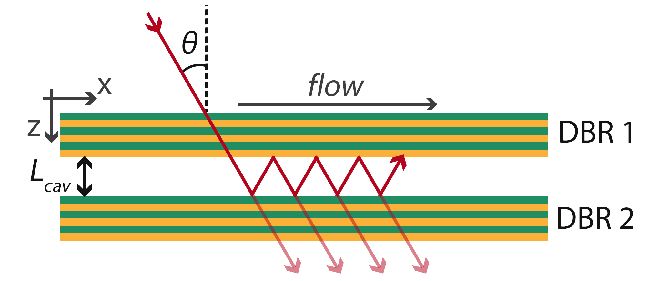
\includegraphics[width=\textwidth]{chap_theory/fig/cavity_geometry.pdf}
    \caption{Photon in a planar microcavity}
    \label{fig:cavity_geometry}
\end{figure}

\textbf{Planar microcavity parameters:}
First, let us consider an electromagnetic field incident at an angle $\theta$ on a planar microcavity made with two mirrors with reflectivities $R_1$ and $R_2$, separated by a distance $L$. The z-axis is normal to the mirrors as shown in \autoref{fig:cavity_geometry}. The phase shift acquired during a single round trip in the cavity is $\Delta \phi (\theta)=2nk_0L\cos(\theta)$, with $n$ the refractive index of the medium and $k_0=2\pi/\lambda$ the wave vector of the field in vacuum. The interference between the multiple reflections sets the resonance condition of the cavity, and the transmission of the field can be written as:

\begin{equation}
    T(\theta)=\frac{R_1R_2}{1+R_1R_2-\sqrt{R_1R_2}\cos(\Delta \phi(\theta)/2)}
    \label{eq:transmission_theta}
\end{equation}

\noindent From this, one can define the decay rate of the field oscillation known as the quality factor:
\begin{equation}
    Q=\frac{\omega_\gamma}{\Delta \omega_\gamma}
    \label{eq:Q}
\end{equation}
with $\omega_\gamma$ the resonance frequency of the cavity and $\Delta \omega_\gamma$ the linewidth of the resonance, which sets the lifetime of the photon in the cavity through $\tau_\gamma=1/\Delta \omega_\gamma$ and depends on the mirrors' reflectivities. Another important parameter describing the cavity is its frequency resolution, which is encoded in the cavity finesse through:

\begin{equation}
    \mathcal{F}=\pi \frac{\Delta \omega_\gamma}{\delta \omega_\gamma} = \pi \frac{\sqrt{R_1R_2}}{1-R_1R_2}
    \label{eq:F}
\end{equation}

where $\Delta \omega_\gamma$ is the Free Spectral Range (FSR) representing the frequency difference between two successive longitudinal modes of the cavity. To achieve strong coupling with the nonlinear medium, the photon needs to stay trapped in the cavity long enough to interact with the medium. In other words, the quality factor of the cavity must be very high, which means using mirrors with high reflectivities. This can be achieved with Distributed Bragg Reflectors (DBR) mirrors.

\begin{figure}[h]
    \centering
    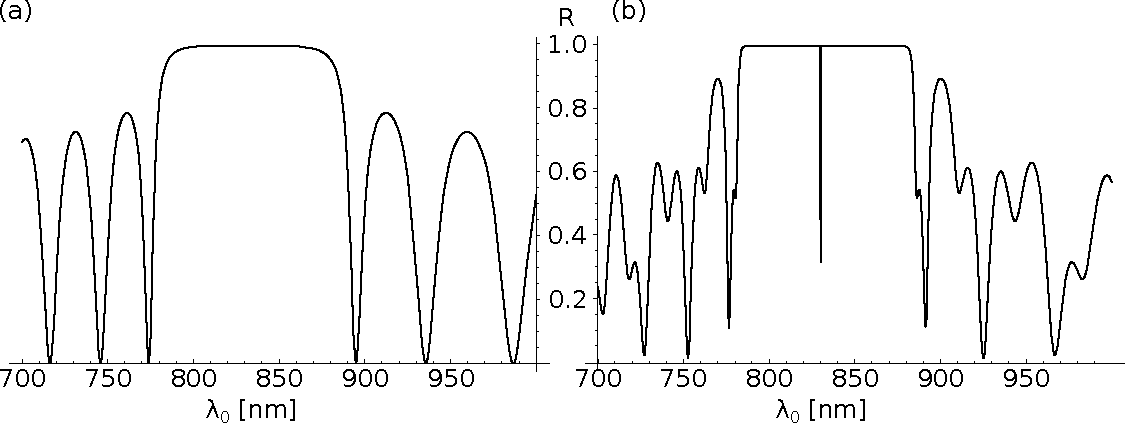
\includegraphics[width=1\linewidth]{chap_theory/fig/DBR.pdf}
    \caption{\textbf{DBR and Fabry-Perot cavity reflectivity.} \textbf{(a)} Reflectivity $R$ of a Bragg mirror of 20 pairs of Ga$_{0.9}$Al$_{0.1}$As/AlAs, illuminated at normal incidence for different wavelengths $\lambda$. The DBR has a reflectivity close to 1 over a large range of wavelengths called the stop-band, centered on $\lambda_0$ = 836 nm by tuning the thickness of each of the mirror layers. \textbf{(b)} Corresponding reflectivity of the optical cavity built from the facing of two DBR mirrors identical to that in (a) and separated by a distance $L_{\mathrm{cav}} = 2\lambda_0 / n_{\mathrm{cav}}$, leading to the appearance of a very narrow resonance at $\lambda_0$. Adapted from ??.}
    \label{fig:DBR}
\end{figure}

\textbf{Distributed Bragg Reflectors.} These reflectors consist of a series of N alternating layers composed of two materials with different refractive indices $n_1<n_2$. This configuration causes partial reflection of the electromagnetic field at each of the N interfaces, resulting in a very high overall reflection coefficient, $R$, which is expressed as follows:

\begin{equation}
    R = \left[  \dfrac{(n_2/n_1)^{2N} - n_f/n_0}{(n_2/n_1)^{2N} + n_f/n_0} \right]^2,
\end{equation}

with $n_0$ and $n_f$ representing the refractive indices of the media before and after the mirrors. \autoref{fig:DBR} illustrates the evolution of $R$ in relation to the wavelength of the electromagnetic field for one DBR mirror used in our system. This mirror is constructed with 20 pairs of $\text{Ga}_{0.9}\text{Al}_{0.1}\text{As}/\text{AlAs}$ layers, having refractive indices $n_2 = 3.48$ and $n_1 = 2.95$ respectively. The reflection coefficient $R$ is 0.9985 across a broad wavelength range, known as the stop-band, centered around a wavelength of $\lambda_0 = 836$ nm. This central wavelength is achieved by setting the thickness of the layers to $d_{1,2} = \lambda_0 / 4n_{1,2}$. The microcavity used in the experiments is built by facing two of those DBR mirrors separated by a distance $L_{\mathrm{cav}}=3\lambda_0/2n_{\mathrm{cav}}$, giving rise to a very narrow resonance at $\lambda_0$ with three field antinodes within the cavity. The parameters of the cavity are summarized in \autoref{DBR_params}.

\begin{center}
    \begin{tabular}{ |p{1.5cm}|p{1.5cm}|p{1.5cm}|p{1.5cm}|p{1.5cm}|p{1.5cm}|}
    \hline
    \multicolumn{6}{|c|}{Fabry-Perot cavity parameters} \\
    \hline
    \hline
    $R_1$ & $R_2$ & $n_1$ & $n_2$ & $n_{cav}$ & $\lambda_0$ (nm) \\
    \hline
    0.9992  &  0.9985 & 2.95 & 3.48 & 3.54 & 836\\
    \hline
    \label{DBR_params}
    \end{tabular}
\end{center}

With the above-described DBR, the cavity has a finesse $\mathcal{F}=2850$ from which we can infer the photon lifetime:
\begin{equation}
    \delta \omega_{\gamma} = \dfrac{\Delta \omega_{\gamma}}{\mathcal{F}} = \dfrac{c}{n_{\mathrm{cav}} L_{\mathrm{eff}}} \dfrac{1-R}{\sqrt{R}},
\end{equation}
where $L_{\mathrm{eff}}= L_{\mathrm{cav}}+L_{\mathrm{bragg}}$ is the effective length of the sample taking into account the penetration of the field in the mirrors.
\begin{equation}
    L_{\mathrm{Bragg}} = \dfrac{\lambda_0}{2} \dfrac{n_1 n_2}{n_{\mathrm{cav}} (n_2 - n_1)}
\end{equation}
which gives $\tau_{\gamma} = \frac{1}{\delta \omega_{\gamma} }= 5$ ps.

\bigskip\noindent
\textbf{Transverse dynamics of the photon.} The energy of the photon within the sample can be written as:
\begin{equation}
    E_\gamma = \dfrac{\hbar c}{n_{\mathrm{cav}}} \sqrt{k_x^2 + k_y^2 + k_z^2}.
\label{free_space_photon}
\end{equation}
The resonance condition of the cavity fixes the photon wavevector along the z component. 

\begin{equation}
    k_z = \dfrac{2\pi n_{\mathrm{cav}}}{\lambda_0}.
    \label{eq:kz}
\end{equation}
In the paraxial approximation $k_x,k_y \ll k_z$, one can expand \eqref{free_space_photon} in terms of $\frac{||\bm{k_{\parallel}}||}{||\bm{k_z}||}$ as:
\begin{equation}
    E_\gamma = \dfrac{\hbar c}{n_{\mathrm{cav}}} \sqrt{k_z^2 + k_{\parallel}^2} = E_0 \left( 1 + (\hbar k_{\parallel })^2 \dfrac{c ^2}{2(n_{\mathrm{cav}} E_0)^2} \right).
    \label{eq:paraxial_photon}
\end{equation}
where $\bm{k_{\parallel}}=\bm{k_x}+\bm{k_y}$ is the wavevector in the transverse plane and $E_0=hc/\lambda_0$ is the photon energy in free space. We can identify the effective mass of the photon by writing \eqref{eq:paraxial_photon} with the usual form of the kinetic energy of a massive particle:

\begin{equation}
    E_\gamma = E_0 + \dfrac{p_{\parallel}^2}{2m_{\gamma}}  
    \label{eq:photon_mass}
\end{equation}
where we identify $m_{\gamma} = \dfrac{\hbar n_{\mathrm{cav}}^2}{\lambda_0 c}$ which is inversely proportional to the second derivative of the energy with respect to $k_{\parallel}$:

\begin{equation}
    \dfrac{1}{m_{\gamma}} = \dfrac{1}{\hbar^2}\dfrac{\partial^2 E_{\gamma}}{\partial k_{\parallel}^2}
    \label{eq:mass}
\end{equation}

\noindent\textbf{Momentum conservation:}
we mentioned the necessity to have a high quality factor to later achieve strong coupling. One could then ask why do we stick to planar designs, which are generally not the best solution to get a high Q factor since they are known to be unstable except for plane waves. The answer lies in the calculation just above. Indeed, the advantage of having a planar design is the translational invariance in the xy plane, which brings $\bm{k_{\parallel}}$ conservation. As a consequence, if one shines a laser with a given $\bm{k_{\parallel}}$, light will behave in the cavity as a massive particle moving at velocity $v_\gamma=\hbar \bm{k_{\parallel}}/m_\gamma$. In the picture of creating a fluid whose flow is controlled, the planar design then appears as a wise choice.

\bigskip\noindent

\noindent\textbf{A direct link between incidence angle and in plane momentum $k_{\parallel}$:}
as shown in \autoref{fig:cavity_geometry} the incidence angle $\theta= (\theta_x, \theta_y)$ of the incoming field is related to the in-plane momentum $k_{\parallel}$ as :

\begin{equation}
    k_{x} = k_0 \sin(\theta_x) \\
    k_{y} = k_0 \sin(\theta_y)
    \label{eq:kpar}
\end{equation}

Controlling the in plane momentum of photons and latter of polaritons then boils down to control the local incidence angle of the field, in other words, the transverse phase of the incoming beam. This is a crucial point for the experiments as it allows to control the flow of the fluid by changing the laser phase.

\bigskip\noindent
\textbf{Conclusion:}
This section revealed how trapping light in a planar microcavity grants it effective mass and lifetime. The next section will explore the semiconducting media that can be inserted into these cavities, especially the bound electron-hole pairs called excitons that can be addressed by the trapped light.


\section{Excitons in Semiconductors}

\subsection{Band theory in brief}

Applying the Schrodinger equation to an atom reveals that the electrons energies can only take discrete values. However, N atoms sufficiently close to each other interact which lift the degeneracy and 
turns each energy state in a set of N separated levels (see \autoref{fig:band_theory}). 
Within a solid material, the density is so high (typicaly $10^{22}$ atoms per cm$^3$) that the spacing between energy levels tends to zero forming a continuous band of energy. 
The electrons fill the band from the lowest energy level up to the Fermi energy. The Fermi energy is the energy of the highest occupied state at zero temperature. 
The band structure of a material is then defined by the energy of the valence band, the conduction band and the band gap between them. The valence band is the highest energy band that is fully occupied at zero temperature, while the conduction band is the lowest energy band that is empty at zero temperature. The band gap is the energy difference between the conduction band and the valence band. 
Determining if a material is a metal, a semiconductor or an insulator is then a matter of comparing the band gap to the Fermi energy.
For metals the conduction band and the valence band overlap, any electric potential difference puts then the electron into motion and create a current. For insulators and semiconducting materials the Fermi energy is in the band gap. For insulators the band gap is typicaly $\sim 3 \ \mathrm{eV}$ making the promotion of an electron to the conduction band highly energy demanding. 
Finally, the semiconductors gap energy is accessible with photons in the visible domain making these materials perfect candidates for controlled light-matter interactions.

\begin{figure}[h]
    \centering
    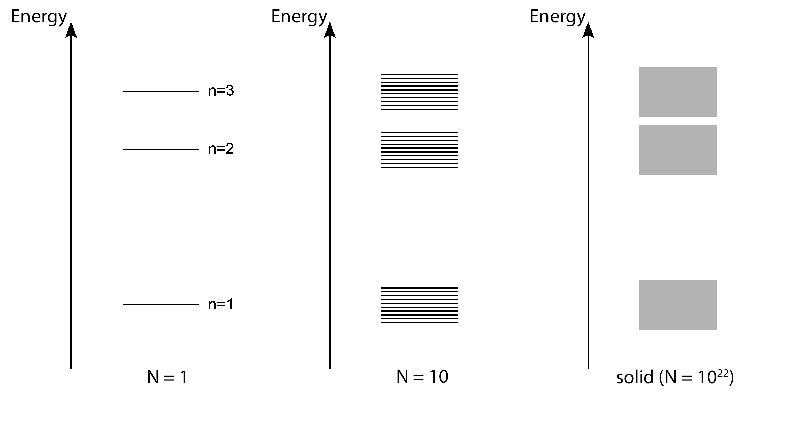
\includegraphics[width=1\linewidth]{chap_theory/fig/band_theory.pdf}
    \caption{\textbf{Energy levels of a set of N atoms.} As N increase the spacing between two successive levels tends to zero and eventually form a continuous band of energy.}
    \label{fig:band_theory}
\end{figure}

\subsection{Band structure of semiconductors}

Finding the exact band structure of a material can be done by solving the Schrodinger equation for an electron in periodic potential.
 The Bloch theorem states that the wave function of such an electron can be written as a plane wave modulated by a periodic function. The periodic function is then expanded in a Fourier series and the Schrodinger equation is solved for each Fourier component. 
 The exact band structure can be rather complicated but a simplified version can be obtained by considering the effective mass approximation \cite{kittel_introduction_2005}. In this picture, the dispersion relation of the electron in the material is typically represented in \autoref{fig:Direct_gap_disp}.
In this case the minimum of the conduction band and the maximum of the valence band are located at the same point in the Brillouin zone. The material is then said to have a direct band gap.
\begin{figure}[h]
    \centering
    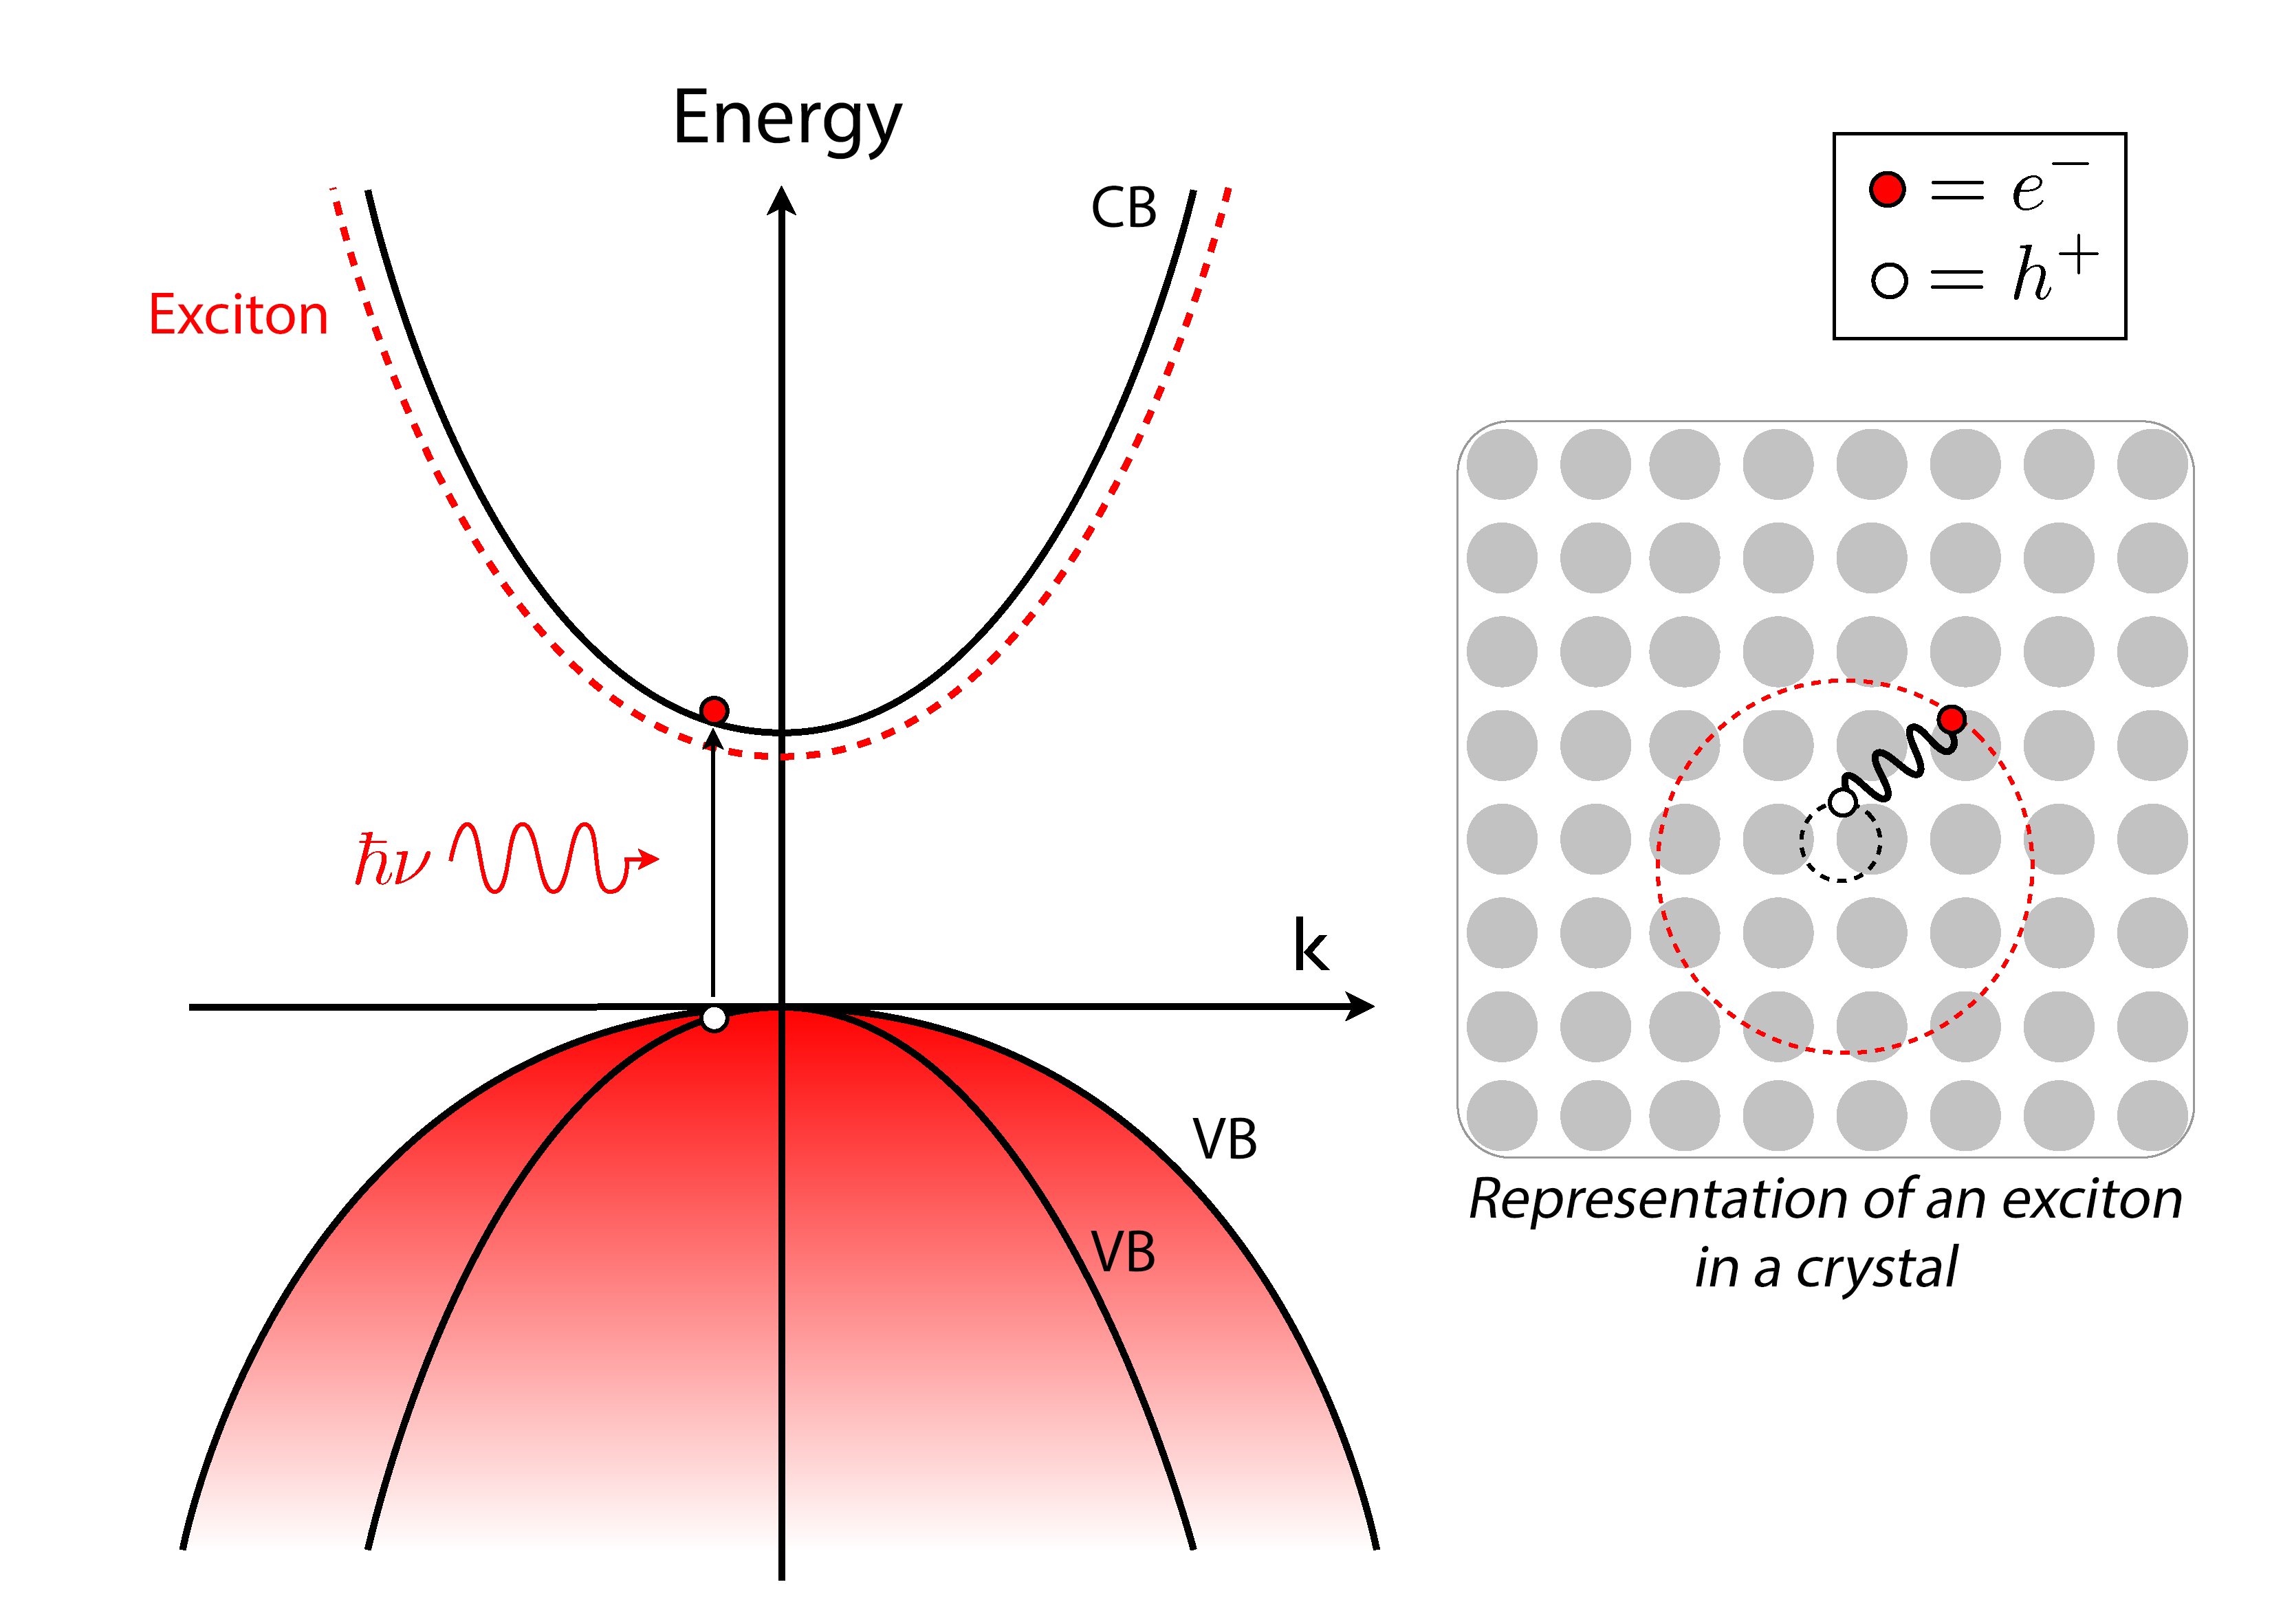
\includegraphics[width=0.8\linewidth]{chap_theory/fig/DirectGapDisp.png}
    \caption{\textbf{Band structure of a direct gap semiconductor.} The black solid line represent the conduction and valence band in a bulk semiconductor. The red dashed lines represent the dispersion relation of an exciton. The filling of the valence band by electrons is represented by the shaded red color.}
    \label{fig:Direct_gap_disp}
\end{figure}


\subsection{Exciton phenomenological approach}

\label{sub:exciton}

As shown in \autoref{fig:Direct_gap_disp} shinning a photon whose energy exceed the gap energy can promote an electron from the valence band to the conduction band through the absorption of a photon. 
The disappearance of the electron in the valence band can be described equivalently as the creation of a virtual particle of opposite charge called hole \cite{Combescot_cooper_excitons_2015}.
 If one scan shine a laser on a semiconductor and ramp up its frequency a narrow absorption peak is observed below the gap energy.  The presence of this peak originate from the coulombic interaction between the created electron and the hole creating a bound state of the material. In terms of energy it's as if the gap energy is reduced by the binding energy of the exciton and the electron lies in a virtual band below the conduction band as represented by the red dashed lines in \autoref{fig:Direct_gap_disp}.
 The exciton energy can then be written as : 

\begin{equation}
    E_{X} = E_g - E_b + \frac{\hbar^2 K^2}{2m_{X}}
\end{equation}

where $E_g$ is the gap energy, $E_b$ the binding energy,  $\hbar \vec{K}$ is the exciton momentum defined as the electron-hole pair center of mass momentum and $m_{X}$ the exciton effective mass which is the sum of the electron and hole effective mass.
Since $E_b$ is the interaction energy between a electron and a hole it is, as we will se in the next section, very similar to the Rydberg energy series of the hydrogen atom, the hole playing the role of the proton. As a consequence, the same electronic structure exist for the exciton : 1s, 2s, 2p, etc state can be observed in the absorption spectrum of the material.
However, the hole is quite different from the proton in the sense that it's actually a collective excitation of all the valence band electrons. Furthermore the exciton is a weakly bound state as the binding energy is typically a few meV. In GaAs or AlGaAs heterostructures which are the materials used in the present work $E_b$ is around 4 meV due to their high dielectric constant $\epsilon_r \sim 12$.
In these kind of samples, excitonic resonances can only be observed at cryogenic temperatures since the binding needs to exceeds the thermal energy $k_B T$ in order to survive the thermal fluctuations. For the above mentionned structures we obtain the condition $T<10$ K for excitons stability.
Another important exciton characteristic is their huge Bohr Radius $a_X= \frac{\epsilon_r \hbar^2}{m_X e^2}= 11.6 \ \mathrm{nm}$ in GaAs which  is much larger then the typical size of a unit crystalline cell $a_0 = 5.65 \SI{1}{\angstrom}$. This means that the exciton wavefunction is delocalized over many unit cells. Such excitons, are called Wannier-Mott and constrast with Frenkel excitons which are localized on a single unit cell and are typically found in organic materials.
 \bigskip\noindent

\subsection{Electron-hole interactions and exciton formation}

Excitons were said to be made of an electron and a hole bound by Coulombic interactions. However, all the interactions in the material are ultimately mediated by valence and conduction band electrons. The rising
of a bound state in such a material is therefore not obvious. In other words moving from a conduction-valence band electrons to a electron-hole picture is not trivial and reveals interesting
feature about the electron-hole interactions that will at the end enable exciton formation. In this section we will first describe all the possible interactions between the electrons of the semiconductor before showing how they can be recasted in terms of electron-hole interactions.

\bigskip
\subsubsection{Electron scattering in semiconductors}
\begin{figure}[h]
    \centering
    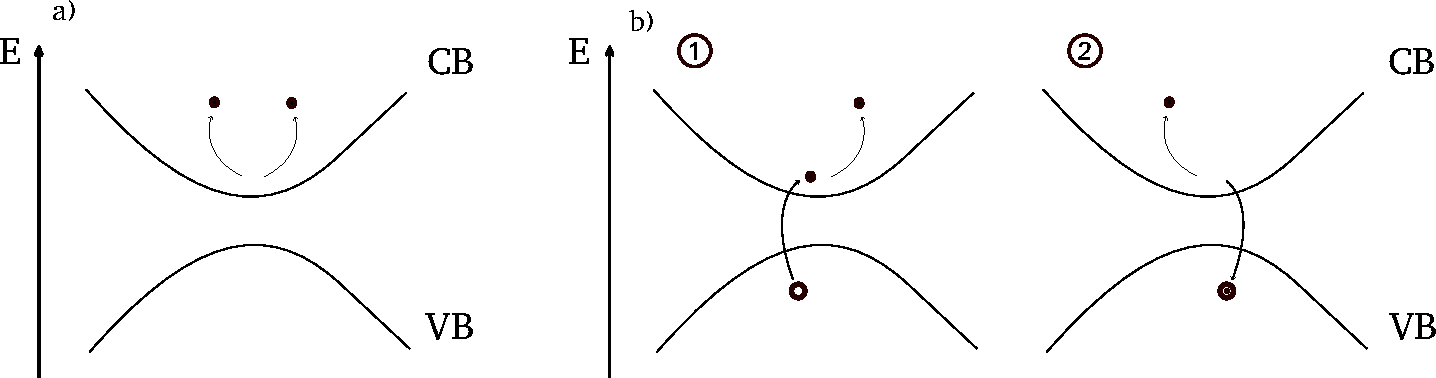
\includegraphics[width=1\linewidth]{chap_theory/fig/intra-inter-band-processes.pdf}
    \caption{\textbf{Drawing representing the scattering between two conduction band electrons.} a) Direct intraband scattering. Filled black dots represent conduction band electrons. b) Two steps scattering involving an electron-hole exchange or creation an annihilation of an exciton, referred as interband scattering.
    The empty black circle represent a valence band hole while the same circle with a small black dot inside stands for a valence band hole filled with an electron which is equivalent to a valence electron. a) and b) share the same
     final state which is a full valence band and two scattered conduction band electrons. Drawing inspired from \cite{Combescot_cooper_excitons_2015}.}
    \label{fig:inter-intra-scat}
\end{figure}


\textbf{Intraband scattering :}
to start with let's consider the direct scattering between two conduction band electrons as presented in \autoref{fig:inter-intra-scat} a). This simple process is referred as intraband scattering since each electron stays in its own band. In the small momentum limit $\mathrm{\textbf{q}}\to 0$ it yields a potential of the form:

\begin{equation}
    V_{\textbf{q}} \simeq \dfrac{4\pi e^2}{L^3 q^2}
\end{equation}
 
\noindent in a sample of size L. This form of potential holds also for the scattering between two valence electrons or between a valence and a conduction band electron that stay in their respective bands.

\bigskip

\textbf{Interband scattering :}
processes in which one or two electrons change band are also possible and are referred as interband scattering. In the case of a single 
interband jump the potential reads $(\frac{q}{\kappa})V_{\textbf{q}}= \dfrac{4\pi e^2}{L^3 q \kappa}$ where $\kappa$ is a dimensionnal factor that depends on the material. It then behaves as $1/q$. When both electrons change band the potential is then $(\frac{q}{\kappa})^2V_{\textbf{q}}$ proportionnal to $q^0$
and thus remaining finite when $q\to 0$. Remarkably, in both the single and two interband jump scenarios, the number of electrons in each band changes by one and two, respectively, making these transitions less likely to occur compared to number-conserving processes.

\bigskip
Indeed, in second order perturbation theory the transition amplitude between an initial state $\ket{i}$ and a final state $\ket{f}$ may be written as :

\begin{equation}
    \Gamma_{i\to f}^{(2)} = \dfrac{2\pi}{\hbar} \bigg \vert \sum_{m} \dfrac{\bra{f}V_q\ket{m}\bra{m}V_q\ket{i}}{E_i - E_m}\bigg \vert^2 \delta(E_f - E_i)
    \label{eq:transition_amplitude}
\end{equation}

\noindent Whenever an electron undergo a band jump the energy cost is of the order of the band gap $E_f - E_i \simeq E_g$. As a consequence the corresponding transition amplitude gets reduced by a factor $\frac{1}{E_g}$ and appears to be negligible.
 However a direct intraband scattering can happen in several interband jumps that will dress the direct Coulomb scattering as shown in \autoref{fig:inter-intra-scat} b) for the case of two jumps. When summing over all possible intermediate state as is \eqref{eq:transition_amplitude} we end up with the same potential as the direct intraband scattering but reduced by dielectric constant factor $\epsilon_{sc}$ that depend on the material.

 
\bigskip




To clarify this idea let us now consider the scattering between a conduction and a valence band electron. 
The same scattering process can also occur in two steps. First, a conduction band electron is scattered in its band while a valence band electron is promoted to the conduction band. Since an electron changes band it brings a potential $V_q(q/\kappa)$. Secondly, 
 the excited electron goes back to the valence band while a valence band electron is scattered in its band yielding again a potential $V_q(q/\kappa)$. This two steps interaction end up with the same initial and final states than direct intraband scattering and the number of electrons in each band is conserved.  
In terms of energy, the two scatterings behaving as $1/q$ potentials the overall potential behaves also as $1/q^2$ but with an additionnal $1/E_{g}$ factor coming from the intermediate interband jumps. More specifically the two steps contribution is : $\left( 4\pi e^2/L^3q^2 \right)\left[ (e^2/L^3\kappa^2)/E_{g}\right]$.  

\bigskip
It is also possible to make it a three steps scattering by adding an intermediate interband exchange after the first step : the previously excited conduction band electron returns to the valence band while a valence band electron is promoted to the conduction band. 
Moe explicitly the process is as follows : 

\begin{itemize}
    \item \textbf{Step 1 :} a valence band electron is promoted to the conduction band while a conduction bandis scattered in its band. The potential reads $V_q(q/\kappa) \propto \frac{1}{q}$ and the energy cost is of the order of $E_g$.
    \item \textbf{Step 2 :} the previously excited conduction band electron returns to the valence band while another valence band electron is excited to the conduction band. The potential read $V_q(q/\kappa)^2 \propto q$ and the energy cost is of the order of $2E_g$.
    \item \textbf{Step 3 :} the excited electron goes back to the valence band while a valence band electron is scattered in its band. The potential read again $V_q(q/\kappa) \propto \frac{1}{q}$ and the energy cost is of the order of $E_g$.
\end{itemize}

\noindent The total energy budget is then : $\left( 4\pi e^2/L^3q^2 \right)\left[ (e^2/L^3\kappa^2)/E_{g}\right]^2$. Remarkably, one might expect the overall potential to scale as $1/E_g^3$  since each step requires at least one electron to change band. However, the structure of perturbation theory ensures that the total energy denominator accounts for the number of coupled interband transitions, rather than treating each step independently. 
Step 2 effectively "couples" the transitions in such a way that two energy denominators are introduced, rather than three independent ones, which explains the 
$1/E_g^2$ dependence. This coupling reflects the fact that intermediate states are shared between adjacent steps in the perturbative sequence.
\bigskip 


\begin{figure}[h]
    \centering
    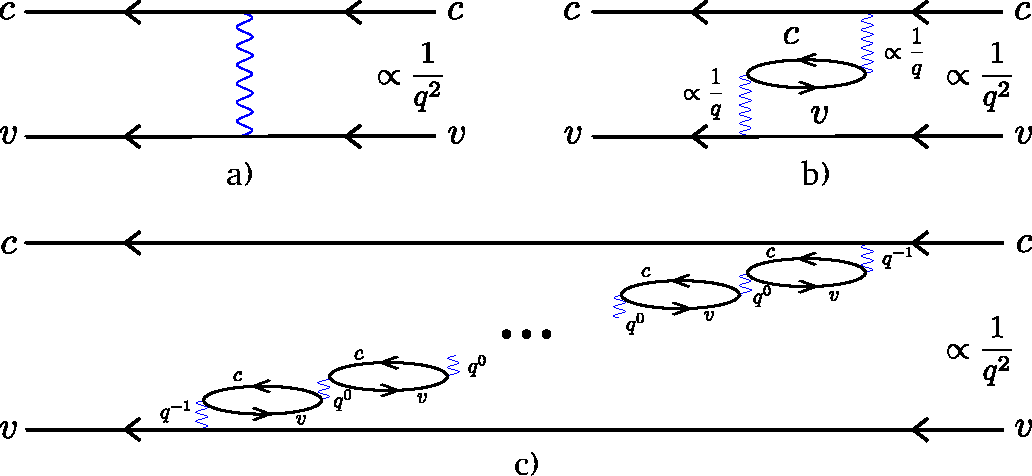
\includegraphics[width=1\linewidth]{chap_theory/fig/intra_band_dressed_bubbles.pdf}
    \caption{\textbf{Feynman diagrams representing an intraband scattering between a conduction and a valence band electron.} a) Direct intraband scattering. The blue wavy lines represent the Coulomb interaction that make the electrons to change states. b) Two steps scattering involving an intermediate interband exchange that is represented by the bubble in the middle.
    c) Multiple steps scattering involving several interband exchanges represented by the numerous bubbles.
    Drawing inspired from \cite{Combescot_cooper_excitons_2015}.}
    \label{fig:intra_bubbles}
\end{figure}

Finally, the number of intermediate states can be arbitrarily increased by adding 'bubbles' of exchange interaction, as illustrated in the Feynman diagram in \autoref{fig:intra_bubbles} b). Each pair of adjacent bubbles represents an interband interaction similar to the one described in Step 2 above. While it conserves the number of electrons in each band, it involves two interband jumps. 
The interaction between two bubbles is then $\propto q^0$ and is finite in the small momentum limit.
By summing the contributions of processes with all possible numbers of bubbles, we obtain an effective Coulomb potential:

\begin{equation}
    V_q = \dfrac{4\pi e^2}{L^3q^2\epsilon_{sc}}
    \label{eq:effective_potential_intraband_scattering}
\end{equation}

where $\epsilon_{sc}$ is a dielectric constant stemming from the infinite sum over the number of bubbles. The discussion that we just made also holds for the intraband scattering between two conduction band electrons or two valence band electrons.
Indeed, it graphically boils down two change the letter of the bands in the Feynman diagrams of \autoref{fig:intra_bubbles} which doesn't change the overall energy budget of the process. Consequently, the potential \eqref{eq:effective_potential_intraband_scattering} is valid for all intraband scattering processes.
Based on the previous discussion we restrict the Coulomb potential that describe any scattering process to interactions that conserve the number of particle in each band, namely the intraband scattering potential between conduction and valence band electrons derived above.
The general form of the potential is then in second quantization :
\begin{equation}
    V_{coul}\simeq \dfrac{1}{2}\sum_{\textbf{q}\neq 0}\Vintra\sum_{\mathbf{k_{1}, k_{2}}}\sum_{\mathrm{i_1,i_2}} a^{\dagger}_{\mathrm{i_{1}},\mathbf{k_1+q}}a^{\dagger}_{\mathrm{i_{2}},\mathbf{k_2-q}}a_{\mathrm{i_{2}},\mathbf{k_2}}a_{\mathrm{i_{1}},\mathbf{k_1}}
\end{equation}

\noindent where $\mathrm{i_1,i_2} \in (c,v)$. The creation operators $a^{\dagger}_{c,\mathbf{k}}$ and $a^{\dagger}_{v,\mathbf{k}}$ create respectively a conduction and a valence band electron with momentum $\mathbf{k}$.
The $\textbf{q}=0$ contribution is not included and treated separately by the wise choice of an average electron-electron potential $V_{e-e}$ that cancels it. More details can be found in the Appendix of \cite{Combescot_cooper_excitons_2015}.
It is worth noting that, in the conduction-valence electron framework, all intraband interactions are identical and repulsive. From this it is not obvious how a bound state like an exciton can arise in the material. However, as we will see in the next section, transitioning to the electron-hole description transforms one of these scattering interactions into an attractive interaction.
 This feature is central to the energy splitting between two types of excitons: bright excitons, which couple to light, and dark excitons, which do not.

\subsubsection{From the conduction-valence electrons to electron-hole picture}

\label{sub:electron_hole_picture}
So far we described the scattering processs within the semiconductor using valence and conduction electrons. However, the exciton results form the binding between a conduction band electron and the absence of a valence band electron that we usually describe as a hole.
While the conduction electron description stays the same, moving from one picture to the other require to define the hole creation operator that account for the removal of a valence band electron or equivalently the creation of a hole in the valence band.


\begin{subequations}
    \label{eq:hole_creation_operators} % Étiquette pour le groupe d'équations
    \begin{align}
        a^{\dagger}_{c,\mathbf{k}} &= a_{\mathbf{k}},\label{eq:electron_operator} \\
        a_{v,\mathbf{k}} &= h^{\dagger}_{\mathbf{-k}},\label{eq:hole_operator}
    \end{align}
\end{subequations}


\noindent where $h^{\dagger}_{\mathbf{-k}}$ creates a hole in the valence band with momentum $-\mathbf{k}$. The - sign 
is imposed by energy and momentum conservation laws. When we substitute the full valence band with a missing electron with momentum $\mathbf{k_v}$ by a hole, the hole needs to have opposite charge $+|e|$, momentum $\mathbf{k_h}=-\mathbf{k_v}$ and energy $E_h(\mathbf{k})=-E_v(\mathbf{k})$ to account for the "absence" of the valence electron. 
In the small momentum limit we have $E_v(\mathbf{k}) = E_{v_0}+ \frac{\hbar^2 k_v^2}{2m_v}$ with $m_v$ the valence electron effective mass that is negative as visible in \autoref{fig:Direct_gap_disp}.
The constraint on the energy $E_h = -E_v$ then imposes $ \frac{\hbar^2 k_h^2}{2m_h} = - \frac{\hbar^2 k_v^2}{2m_v}$ making the effective mass of the hole positive. Its charge and mass being positive it can then undergo attractive interactions 
with a conduction band electron and eventually form an exciton. We already see how describing the valence band with hole instead of electrons can predict the formation of bound state.
Let us now look how this feature arise from a microscopic point of view. The full crystal hamiltonian is :

\begin{equation}
    \Ham =  \Ham_0 + V_{coul}
    \label{eq:crystal_hamiltonian}
\end{equation}

\noindent with $\Ham_0$ the free electron hamiltonian and $V_{coul}$ the Coulomb interaction between electrons. The free electron hamiltonian reads :

\begin{equation}
    \Ham_0 = \sum_{\mathbf{k}} E_c(\mathbf{k}) a^{\dagger}_{c,\mathbf{k}}a_{c,\mathbf{k}}+\sum_{\mathbf{k}} E_v(\mathbf{k}) a^{\dagger}_{v,\mathbf{k}}a_{v,\mathbf{k}}
    \label{eq:free_electron_hamiltonian}
\end{equation}

\noindent where $E_c(\mathbf{k})$ and $E_v(\mathbf{k})$ are the conduction and valence band energies respectively. The Coulomb interactions part can be decomposed in the following way :

\begin{equation}
    V_{coul} = V_{cc} + V_{vv} + V_{cv}
    \label{eq:coulomb_interaction}
\end{equation}
Using the newly defined operators together with fermionic commutation relation $a^{\dagger}_{i,\textbf{k}}a_{i,\textbf{k}}= 1-a_{i,\textbf{k}}a^{\dagger}_{i,\textbf{k}}  $ the different scattering potentials are modified as we now show. 

\begin{itemize}
    \item The one body hamiltonian reads : 
    \begin{equation}
    \Ham_0 = \sum_{\veck}E_v(\veck)+ \sum_{\veck}E_c(\veck) a^{\dagger}_{\veck}a_{\veck} + \sum_{\veck}-E_v(\veck) h^{\dagger}_{\veck}h_{\veck}.
    \end{equation}

    \item The scattering between two conduction band electron is the same as before :
    \begin{equation}
    V_{cc} = \dfrac{1}{2}\sum_{\textbf{q}\neq 0}V_{\mathbf{q}} \sum_{\mathbf{k_{1}, k_{2}}} a^{\dagger}_{\mathbf{k_1+q}}a^{\dagger}_{\mathbf{k_2-q}}a_{\mathbf{k_2}}a_{\mathbf{k_1}} \equiv V_{ee}
    \label{eq:cc_interaction}
    \end{equation}

    \item The scattering between two valence band electrons splits into three terms :
    \begin{equation}
    V_{vv}=-\dfrac{N_v}{2}\sum_{\veck \neq 0}V_{\veck} + \sum_{\veck}\hkdag\hk\sum_{\veck'\neq \veck}V_{\veck'-\veck}+V_{hh}.
    \label{eq:vv_interaction}
    \end{equation}

    The first term is constant and account for repulsive exchange interaction between all valence electrons. The second term comes from the scattering between a valence electron with wavevector $\veck$ and all the other valence electrons.
    It adds a shift to the hole kinetic energy $E_h = -E_v$ that appears in the one body hamiltonian $\Ham_0$. 
     The last term is the hole-hole interaction that is repulsive and is the same as the valence electron-electron interaction with opposite wavevectors : 
    \begin{equation}
    V_{hh} = \dfrac{1}{2}\sum_{\textbf{q}\neq 0}V_{\mathbf{q}} \sum_{\mathbf{k_{1}, k_{2}}} h^{\dagger}_{\mathbf{k_1+q}}h^{\dagger}_{\mathbf{k_2-q}}h_{\mathbf{k_2}}h_{\mathbf{k_1}} 
    \label{eq:hh_interaction}
    \end{equation}

    \item Finally, scattering between a conduction and a valence band electron is :
    \begin{equation}
    \label{eq:cv_interaction_in_cv_picture}
    V_{cv} = \sum_{\textbf{q}\neq 0}V_{\mathbf{q}} \sum_{\mathbf{k_{1}, k_{2}}} a^{\dagger}_{c,\mathbf{k_1+q}}a^{\dagger}_{v,\mathbf{k_2-q}}a_{v,\mathbf{k_2}}a_{c,\mathbf{k_1}}.
    \end{equation}
    Using that for non zero momentum transfer $[a^{\dagger}_{v,\mathbf{k_2-q}}, a_{v,\mathbf{k_2}}] = 0$ and introducing $\mathbf{k_2'} = -(\mathbf{k_2-q})$ the potentials in terms of electron-hole reads :
    \begin{equation}
        V_{cv} = -\sum_{\textbf{q}\neq 0}V_{\mathbf{q}} \sum_{\mathbf{k_{1}, k_{2}'}} a^{\dagger}_{\mathbf{k_1+q}}h^{\dagger}_{\mathbf{k_2'-q}}h_{\mathbf{k_2'}}a_{\mathbf{k_1}} \equiv V_{eh}.
    \label{eq:eh-interaction}
    \end{equation}

\end{itemize}
The latter require a special attention since it exhibits an attractive interaction and reveals the possibility of excitons formation which was not obvious in the conduction-valence electron picture.
\bigskip

\noindent \large \textbf{Spin conservation in electron scattering } \normalsize
\bigskip


Scatterings processes mediated by the Coulomb interactions conserve the spin of the electron for both interband and intraband scatterings. As a consequence,
the interactions between electons and holes that we just exhibited are also spin preserving. The latter has important consequences to determine
selection rules when looking at optical excitation of an electron-hole pair. 

\bigskip

\indent So far we demonstrated that replacing the full valence band by a hole looks quite convenient since it allow to forget about all the valence band electrons and exhibits the possibility of bound state formation. However, it must be done with caution
since the remaining valence band electrons undergo the many intraband scattering processes described in the section and reduce the effective Coulombic intraband interaction by 
a factor $1/\epsilon_{sc}$. Remarkably, the intraband scatterings between valence and conduction band electrons $V_{cv}$ are at the origin of the attractive electron-hole interactions while valence-valence interactions are responsible for the shift in the hole kinetic energy as expressed by \autoref{eq:vv_interaction}.
Let us now explain how the aforementioned electron-hole attractive interactions can lead to exciton formation.

\subsubsection{The electron-hole hamiltonian}
\label{e-h_hamiltonian}

If we restrict the previous description to a one pair subspace namely to the interactions between a single electron and a single hole, electron-electron and hole-hole
interactions can be safely dropped since they require two holes or electrons. The one pair hamiltonian then reads : 


\begin{equation}
    \begin{align}
    \Ham_{eh} &= \Ham_e + \Ham_h + V_{eh}, \\
              &= \sum_{\veck}E_c(\veck) a^{\dagger}_{\veck}a_{\veck} + \sum_{\veck}E_h(\veck) h^{\dagger}_{\veck}h_{\veck} - \sum_{\textbf{q}\neq 0}V_{\mathbf{q}} \sum_{\mathbf{k_{1}, k_{2}}} a^{\dagger}_{\mathbf{k_1+q}}h^{\dagger}_{\mathbf{k_2-q}}h_{\mathbf{k_2}}a_{\mathbf{k_1}}.
    \label{eq:electron_hole_hamiltonian}
    \end{align}
\end{equation}
Wannier exciton are the solutions $\ket{x}$ of the eigenproblem :
\begin{equation}
    (\Ham_e + \Ham_h + V_{eh})\ket{i}= E_i\ket{i}
    \label{eq:exciton_eigenproblem}
\end{equation}
with eigenvalue $E_i$.
At this level the hamiltionian is very general and describe two coupled harmonic oscillators. Without going into details, this problem can be solved by following the same procedure as in classical mechanics.
The core of the derivation consists in decoupling the two oscillators by introducing new coordinates that are the center of mass and relative coordinates. Since Coulombic interaction conserve momentum, the total momentum of the
electron-hole pair $k_e+k_h$ stays constant and is equal to the exciton center of mass momentum $\mathbf{Q}$. Namely, we define :

\begin{subequations}
    \begin{align}
        \mathbf{Q} &= \mathbf{k_e} + \mathbf{k_h}, \\
        \mathbf{q} &= \gamma_h\mathbf{k_e} - \gamma_e\mathbf{k_h},
    \end{align}
\end{subequations}
where $\gamma_e =1- \gamma_h= m_e/(m_e+m_h)$ is the reduced mass ratio and $\mathbf{q}$ is the relative motion momentum. We then define the creation operator that creates an exciton $\ket{x}$ in state $(\mathbf{Q_i}, \nu_i)$ in terms of electron and hole operators : 

\begin{equation}
    b^{\dagger}_{\mathbf{Q_i},\nu_i} =  \sum_{\mathbf{p}}f_{\mathbf{p}}^{\nu_i}a^{\dagger}_{\gamma_e\mathbf{Q_i}+\mathbf{p}}h^{\dagger}_{\mathbf{-p+\gamma_h\mathbf{Q_i}}}
\end{equation}
\bigskip
\noindent where $f_{\mathbf{p}}^{\nu_i} = \bra{\mathbf{p}}\ket{\nu_i}$ is the relative motion wave function. Let us show that the states $\ket{\nu_i}$ are the eigensolutions of a Hydrogen like problem $\nu_i$ being then related to the first quantum number of an electron orbitals. Injecting $\ket{x}= b^{\dagger}_{\mathbf{Q_i},\mathbf{q_i}}\ket{0}$, $\ket{0}$ being the vacuum state in 
\autoref{eq:exciton_eigenproblem} we obtain $\Ham_{eh}$ in a diagonal form :

\begin{equation}
    \begin{align}
    \Ham_{eh}b^{\dagger}_{\mathbf{Q_i,\nu_i}}\ket{0} = \sum_{\mathbf{p}}  \left\{\left(E_g + \dfrac{\mathbf{Q_x}^2}{2m_X} + \dfrac{\mathbf{p_x}^2}{2\mu_X} \right)f_{\mathbf{p}}^{\nu_i} - \sum_{\mathbf{q}\neq 0} V_\mathbf{q}f_{\mathbf{p-q}}^{\nu_i}\right\}a^{\dagger}_{\mathbf{p+\gamma_e\mathbf{Q_i}}}h^{\dagger}_{\mathbf{-p+\gamma_h\mathbf{Q_i}}}\ket{0}
    \end{align}
\end{equation}
whose eigenstates are $b^{\dagger}_{\mathbf{Q_i,\nu_i}}\ket{0}$ with energy $E_{X_i} = E_g + \frac{\mathbf{Q_i}^2}{2M_X} + E_{b}^i$ if and only if $f_{\mathbf{p}}^{\nu_i}$ are solution of the Hydrogen-like problem : 

\begin{equation}
    \dfrac{\mathbf{p}^2}{2\mu_X}f_{\mathbf{p}}^{\nu_i} -\sum_{\mathbf{q}\neq 0} V_\mathbf{q}f_{\mathbf{p-q}}^{\nu_i} = E_b^if_{\mathbf{p}}^{\nu_i}
    \label{eq:hydrogen_like_problem}
\end{equation}
 where $\mu_X^{-1}= m_e^{-1}+m_h^{-1}$ is the relative motion mass and $m_X = m_e+m_h$ the total mass. The exciton then appears as a bound state of the electron-hole pair with a binding energy $E_{b_i}$ whose center of mass 
 is delocalized as a plane wave with momentum $\mathbf{Q}$. The binding energies $E_b^i$ follows a Rydberg series $E_b^i = -\dfrac{R_X}{i^2} $ where $R_X$ is the Rydberg constant of the exciton as defined in \autoref{sub:exciton}
In the following section we will see how the excitons interact with light.

 \subsection{Exciton-photon interaction in bulk semiconductor:} 
 \label{sub:exciton_photon_interaction}
The creation of an exciton can be mediated by the absorption of a photon by the material. On the other the annihiliation of a exciton can lead to photon emission.
As a start we describe this interaction with an usual electron-photon Hamiltonian in first quantization:


\begin{equation}
    \Ham_{dip} = -e \dfrac{\mathbf{p_e} \cdot \mathbf{A}}{m_e},
\end{equation}

with $\mathbf{p_e}$ the momentum operator of the electron and $\mathbf{A}$ the potential vector of the electromagnetic field. Before going further let us have a look at what the symetries of this Hamiltonian imply based on the Noether theorem.

\begin{itemize}
    \item \textbf{Total momentum conservation :}  translational invariance of the system implies that the total momentum of the system is conserved. The absorption of a photon with momentum 
    $\hbar \vec{k_c}$ will create an exciton with the same momentum.
    \item  \textbf{Total angular momentum conservation :} rotational invariance of the system implies that the total angular momentum of the system is conserved along the interaction.
\end{itemize}

The second point raises the question of the possible values that the exciton angular momentum can assume. To answer this question we need to get back to its 
microscopic constitutive particles : a conduction band electron and a hole in the valence band. In usual semiconductors a conduction band electron has an orbital angular momentum ($L=0 , L_z=0$) while a valence band electron yields ($L=1 , L_z=(+1,0,-1)$) (see \cite{kittel_introduction_2005}).
Since $J_z = J_z + S_z$ and the electron spin is $S_z = \pm 1/2$ we obtain for the valence band $J_z^{v} = (3/2, 1/2, -1/2, -3/2)$ and for the conduction band $J_z^{c} = \pm 1/2$. If we now move to the electron-hole picture the electron angular momentum remains unchanged $J_z^{e}=J_z^{c}= \pm 1/2$ while the hole angular momentum is the opposite of the valence band electron $J_z^{h} = -J_z^{v}=(3/2, 1/2, -1/2, -3/2)$.
 The exciton angular momentum is then $J_z = J_z^{e} + J_z^{h} = (-2,-1,0,1,2)$. We can thus distinguish \textbf{bright} excitons with $J_z = (-1,0,1)$ that couple to light with polarization $\pi , \sigma_+ , \sigma_-$ and \textbf{dark} excitons with $J_z = (-2,2)$ that do not couple to light. 
In the latter case the spin of the electron and the hole are aligned : $J_z= \pm 2$ excitons are made of $\pm1/2$ electrons and $\pm3/2$ holes. It means it corresponds to a situation in which the valence band electron flipped spin when it got promoted to the electron band. Yet, dark excitons can subsequently not undergo interband transitions that are spin preserving as mentionned in \autoref{sub:electron_hole_picture}. 
On the other hand, bright excitons result from interband transitions since both photon absorption and emission involve an electron changing band. In the framework of polariton which involve exciton creation through light one could think that since
Coulomb inter and intraband scatterings are spin preserving, dark excitons are of no interest and won't play any role in the system. However, we will see that dark excitons can be created from bright excitons thanks to exchange carrier.
that only bright excit



\subsection{Exciton in 2D quantum well}

Let us now get closer to the situation encoutered in the sample used in the experiment. In such microcavities, excitons are confined in a planar quantum well 
which are made by stacking layers of semiconductor materials with different band gaps. The confinement in the plane is then ensured by the potential barrier between the layers.
In our case a quantum well is made of InGaAs placed in between two layers of GaAs. InGaAs has a smaller band gap than the bulk GaAs because of the p-fraction of InAs dopping as shown in \autoref{fig:sc_quantum_well} (b). 
Both electrons and holes then remain confined in the region where the band gap is the smallest (see \autoref{fig:sc_quantum_well} (a)).
By repeating this "sandwiching" procedures it is possible to create many QW heterostructures as we shall see latter.
\begin{figure}[h]
    \centering
    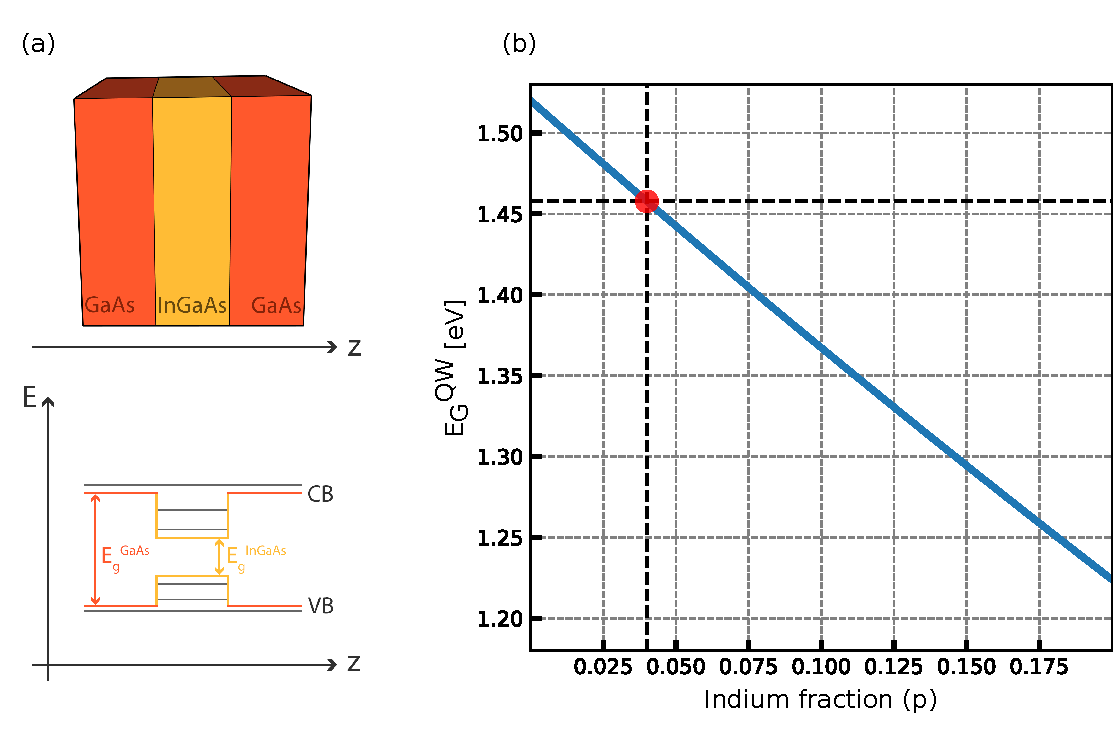
\includegraphics[width=0.8\linewidth]{chap_theory/fig/InGaAs.pdf}
    \caption{\textbf{Schematic representation of a quantum well heterostructure.} a) Representation of a planar quantum well made of InGaAs placed in between two layers of GaAs. The confinement in the plane is ensured by the gap energy difference between the layers.
    b) Gap energy of the InGaAs quantum well as a function of the dopping fraction of Indium. The red dot represent the dopping in sample used in the experiment : $E_g^{InGaAs} = 1.46 eV < E_g^{GaAs} = 1.52 eV$.}
    \label{fig:sc_quantum_well}
\end{figure}

Assuming the same geometry than the above figure the electron-hole hamiltonian taking into account the potential barrier is written in first quantization as :

\begin{equation}
    \Ham = E_g^{QW} + \dfrac{\mathbf{p}^2_e}{2m_e} + \dfrac{\mathbf{p}^2_h}{2m_h} - \dfrac{e^2}{\epsilon_{sc}|r_e-r_h|}+V_e(z_e)+V_h(z_h)
\end{equation}
where z is the growth axis of the quantum well and $V_e(z_e)$ and $V_h(z_h)$ are the potential barriers felt by the electron and the hole respectively, $r_e$ and $r_h$  are the electron and hole spatial coordinates. 
The system is invariant under translation in the $xy$-plane the excitons in plane wavevector $k_{\parallel}$ can then take any value while the confinement in the $z$-direction quantize the corresponding component of the wavevector $k_z$. 
This problem is treated by writting the exciton wavefunction $\Psi(x,y,z)$ as a two components product :

\begin{equation}
    \Psi(x,y,z) = \psi(x,y,z)\phi(z).
    \label{eq:2D_exciton_wavefunction}
\end{equation}

The Schrodinger equation is then solved separately for $\psi(x,y)$ and $\phi(z)$. 
The confinemnt in $z$-direction is treated as a very basic quantum box problem. The electron and hole energies are then quantized as :

\begin{equation}
    E_n^{e,h} = \dfrac{(\pi^2 n^2\hbar^2}{2m_{e,h}L_z^2}
    \label{eq:QW_energy_levels}
\end{equation}

where $L_z$ is the width of the quantum well.

To determine the in-plane wavefunciton we follow the same procedure than for the exciton eigenproblem in the 3D case.
The exciton is again a correlated pair whose center of mass is delocalized as a plane wave with momentum $\mathbf{Q} = \hbar \kpar$. The correspondig energy is then  :

\begin{equation}
    E_X^{xy} = E_g^{QW} + \dfrac{\mathbf{\hbar k_{\parallel}}^2}{2m_X} - \dfrac{R_X^{QW}}{n^2}
\end{equation}
provided that we defined a new Rydberg constant $R_X^{QW}$ taking into account the confinement in the $z$-direction. Remarkably, due to confinement the Bohr radius $a_X^{QW}$
of the QW exciton is twice smaller than the bulk exciton Bohr radius. This is a direct consequence of the confinement that increases the electron-hole wavefunctions overlap and thus the binding energy of the exciton. The exciton total energy is then : 

\begin{equation}
    E_X(\kpar) = E_g^{QW} + E_n^{e} + E_n^{h} +  \dfrac{\mathbf{\hbar k_{\parallel}}^2}{2m_X} - \dfrac{R_X^{QW}}{n^2}
    \label{eq:2D_exciton_energy}
\end{equation}
The design of the sample used in the experiement is done such as the n=1 level is sufficiently far form the next level that we can restrict our description to 
the first 1s exciton state. In the following we will therefore drop the n index by setting it to one.

\bigskip


\noindent \textbf{Bosonic nature of excitons.} Since an exciton is made of two fermions its pseudo spin is an integer. However, when reaching regimes of high excitons densities
the fermionic nature of their microscopic constitutives can no longer be neglected. The composite nature of excitons can then be safely dropped provided that the exciton density per unit area 
is such as $n_X(a_X^{QW})^2 \ll 1$. This condition state that the average distance between excitons is much larger than the exciton Bohr radius. In this regime the excitons can be treated as bosons, namely : 


\begin{equation}
    [b_{\mathbf{k}}, b^{\dagger}_{\mathbf{k}}] = 1 - O(n_X(a_X^{QW})^2) \simeq 1
    \label{eq:exciton_bosonic_nature}
\end{equation}

\bigskip



\noindent \textbf{Optical selection rules in the planar quantum well.}In bulk semiconductors, a single exciton mode couples exclusively to a single photon mode. In quasi-two-dimensional systems, due to the breaking of translationnal invariance in the growth direction $z$ the momentum
conservation during a photon absorption or emission remains valid only for the in-plane component, the $z$-component being fixed by the quantum well width.
Accordingly, an exciton with wavevector $\mathbf{k}_X=(\kpar^X, k_z^X)$ will interact with a photon with the same in plane wavevector but with any value of $k_z^\gamma$. 
There is thus a density of states for radiative decay given by (see \cite{weisbuch_microcavities_1996}):

\begin{equation}
    \rho_{2D}(\kpar, \hbar \omega) \equiv \sum_{k_z}\delta(\hbar\omega - \dfrac{\hbar c}{n_{QW}} \sqrt{\kpar^2+ k_z^2})\propto \dfrac{\hbar\omega}{\sqrt(k_0^2-\kpar^2)}\mathbf{\Theta}(k_0-\kpar)
    \label{eq:2D_dos}
\end{equation}
where where $n_{QW}$ is the refractive index in the QW, $k_0 = n_{QW}\omega/c$ is the wavevector of the photon in the material and $\Theta$ is the Heaviside step function. 
Only states with $|\kpar|<k_0$ can couple to light giving rise again to two class excitons.
\begin{itemize}
    \item States with $|\kpar^X|<k_0$ that couple to light. These states have a finite radiative lifetime $1/\gamma_X$ given by the Fermi Golden rule. They lie on the left of the
    light cone in the $\kpar-\omega$ plane.
    \item States with $|\kpar^X|>k_0$ that do not decay radiatively. They lie on the right of the photon line in the the $\kpar-\omega$ plane.  They are analog to surface
    modes as they have a vanishing electric field far from the QW. These states join the previously described excitons that could not couple to light because of their spin configuration to form
    a wider class of "dark" excitons.
\end{itemize}
This stands in contrast to bulk semiconductors, where a single exciton mode couples exclusively to a single photon mode.
Nevertheless, if we also 
impose energy conservation between the exciton and the photon mode the maximum in-plane wavevector of radiative excitons gets modified and depend on the exciton energy.
To see this let us consider an inital state made of an exciton of overall energy $E_X(\kpar^X)$ and zero photon and a final state made of a single photon with energy $E_\gamma(\kpar^{\gamma})= \frac{\hbar c}{n_{QW}} \sqrt{(\kpar^\gamma)^2+ (k_z^\gamma)^2}$ and no exciton.
The energy conservation of this process reads :

\begin{subequations}
    \begin{align}
    E_X(\kpar^X)&= E_\gamma(\kpar{\gamma}) \\
    E_X^{QW} + \dfrac{(\hbar\kpar^X)^2}{2m_X}  &= \dfrac{\hbar c}{n_{QW}} \sqrt{(\kpar^\gamma)^2+ (k_z^\gamma)^2},
    \end{align}
    \label{eq:energy_conservation}
\end{subequations}
in which we set $E_X^{QW} = E_g^{QW}+ E_X^{1s}= E_g^{QW} + E_1^{e} + E_1^{h}-R_X^{QW}$. Injecting the in-plane momentum 
conservation and imposing ${k_z^\gamma}^2 \geq 0$ for the photon field to be propagative the above condition restricts the exciton that can couple to light through :

\begin{equation}
    |\kpar^X| \leq \dfrac{cm_X}{n_{QW}\hbar}\left(1+\sqrt{1-\dfrac{4n_{QW}E_X^{QW}}{m_Xc^2}} \right).
    \label{eq:k_max}
\end{equation}
Since $E_X^{QW}$ can be negleted with respect to the exciton mass energy $m_Xc^2$ the above condition taken at first order gives :

\begin{equation}
    |\kpar^X| \leq \dfrac{n_{QW}E_X^{QW}}{\hbar c}.
    \label{eq:kmax_approx}
\end{equation}


\noindent Excitons with higher wavevector are than forbidden to exchange energy with light. However, in our case we have $E_X^{QW} \simeq 1.485  /  meV$ and $n_{QW} \simeq 3.5$ leading to $|\kpar^X| \leqslant 30 / \mu m^{-1}$ which is way beyond
the values adressed in the experiment. Now that the exciton formation is well etablished let us have a look at the mechanisms that can lead them to interact.
 

\subsection{Exciton-exciton interaction}
\label{sub:exciton_exciton_interaction}

The scope of this section is to answer the question of what can lead two excitons in states $(i,j)$ to end up in states $(f,g)$. Obviously, direct
coulomb interactions between the excitons constitutive is an unambiguous valid answer. Nonetheless, an interaction giving the same result can also occur in the absence of any Coulomb interactions via pure carrier exchange.
Namely, excitons $i$ and $j$ can exchange either their electron or hole. The latter is a direct consequences of the Pauli exclusion principle stating that two fermions cannot occupy the same quantum state. 


\subsubsection{Coulomb interaction}

As explained in the previous section, holes and electrons undergo Coulomb interaction. As a consequence, the interaction
between two excitons $(e_1,h_1)$ and $(e_2,h_2)$ consist of $V_{e_1e_2}+V_{h_1h_2}+V_{e_1h_2}+V_{h_1e_2}$. However, if the exciton were made of $(e_1,h_2)$ and $(e_2,h_1)$ the cross term in the interaction potentail would be replaced
by $V_{e_1h_1}+V_{e_2h2}$. Because there are different possible ways to form excitons, the total interaction energy depends on the specific pairing choice.
This makes it impossible to define a single, clean exciton-exciton interaction potential that works in all cases.
Hence, treating them as pure bosons with a simple interaction potential fail because the effective exciton-exciton potential is not unique and depends on the microscopic way the excitons are formed.
Nevertheless, it is clear that, through Coulomb interaction, excitons can change states and thus interact in the most general sense. This being said, we will as experimentalist, focus on the most 
important scattering process that is actually coming from exchange carrier among excitons and that is a unique feature of composite particle.

\subsubsection{Fermionic exchange interaction}

Let us consider two excitons $X_1=\ket{\mathbf{k_e},\mathbf{k_h}}$ and $X_2=\ket{\mathbf{k_e}',\mathbf{k_h}'}$. If their wavefunction
start to overlap the two electrons for example might see their qunatum state becaming almost equal which is forbidden by the Pauli exclusion principle. To regularize this situation 
the exciton can exchange their carrier to form $X'_1=\ket{\mathbf{k_e}',\mathbf{k_h}}$ and $X'_2=\ket{\mathbf{k_e},\mathbf{k_h}'}$. This is might look counterintuitive since exchanging two particles in the same quantum state doesn't seem to solve the problem. However,
it's truly the exchange process itself put together with wavefunction symmetries that modify the quantum state configuration to avoid Pauli principle violation.
Take two indistinguishable particles, in state $\psi_a$ and $\psi_b$ in a 1D system  \cite{CCT_tome2}. Normalization consideration aside, the wavefunction of the system can be written in two ways : $\psi_{ab} =\psi_a(x_1)\psi_b(x_2) \pm \psi_a(x_1)\psi_b(x_2)$.
Depending on the plus or minus sign, the wavefunction is symmetric or antisymmetric under position exchange. The two different configurations imply different physics.
For instance the mean value of the particle interdistance is :

\begin{equation}
    \langle(x_1-x_2)^2\rangle = \langle x_1^2\rangle + \langle x_2^2\rangle \mp 2\langle x_1x_2\rangle ,
\end{equation}

provided the wavefunctions overlap $\langle x_1x_2\rangle\neq0$, the expected value is decreased for bosons and increased for fermions. Although, it seems to act 
as a force repelling or attracting particles, it is rather a geometrical constraint arising from the Pauli principle and the quantum nature of the particle at stake.
This is precisely what happend during carrier exchange and can, at the end, lead to scattering processes between excitons. Forgetting about this interaction ad try to fully bosonize excitons would then be a mistake \cite{ciuti_carrier_exchanges_1998}.
As an example, some features experimentally measured like exciton stark effect, precisely needs to put exchange carrier on the table to be understood \cite{exciton_stark_VonLehmen_86,exciton_stark_Mysyrowicz_86,joffre_m_subpicosecond_1987}.
Furthermore, in a 2D quantum well system this scatterings are dominant at larger scale while direct Coulomb interactions are dominant at scales smaller than the Bohr radius of
excitons. Therefore, by considering only radiative modes, i.e. dynamics occuring on scales much larger than the Bohr radius of
excitons $ka_X\ll 1$, Coulomb interactions can be neglected. Despite all the differences with true bosons above mentionned and the hot debates still going on about polaritons interactions \cite{Combescot_2007_exact_pol_pol_interactions,I_frerot_PRX_2023} this enable us, as experimentalist, to escape from ambiguity and write the main exciton-exciton potential that 
will be relevant in the experiment reported in this work. Written in momentum space this exciton-exciton potential $V_{XX}(\kvec)$ appear as four body contact interaction \cite{Rochat2000}. The corresponding hamiltonian follows as :


\begin{equation}
    \Ham_{XX} = \dfrac{1}{2}\sum_{\kvec, \kvec', \vec{q}} V_{XX}(\vec{q}) \hat{b}^\dagger_{\kvec+\vec{q}} \hat{b}^\dagger_{\kvec'-\vec{q}} \hat{b}_{\kvec} \hat{b}_{\kvec'}.
\label{exciton_interaction_ham}
\end{equation}

The potential $V_{XX}(\vec{q})$ is a function of the exchanged momentum $\vec{q}$. However, it can be approximated by a constant in the limit of low wavevectors since, being four order of magnitude heavier than microcavities photons, their varies only slightly with $\kvec$ in the range of the photon wavevector that excite them. Therefore $V_{XX}$ can be assumed constant. The numerical calculation gives $A \times V_{XX}\simeq$ 3 $\mu$eV$\cdot \mu$m$^{2}$ for our InGaAs system.
\begin{equation}
    V_{XX} = \dfrac{e^2 a_X^{QW}}{\epsilon A},
\end{equation}

with $A$ the quantization area equal to the  quantum well surface. The numerical calculation gives $A \times V_{XX}\simeq$ 3 $\mu$eV$\cdot \mu$m$^{2}$ in our GaAs-InGaAs system.

\bigskip

\textbf{Dark excitons creation through carrier exchange.}

As discussed in \autoref{sub:exciton_photon_interaction} electron-hole pairs with a total spin of $\pm1$ are coupled to $\sigma\pm$ photons, meaning that photon absorption leads to the creation of only bright exciton states $\pm1$. However, dark exciton states can also be present in the system, arising from fermion exchange processes.
Namely, fermion exchange between two bright excitons $(+1,1)$ made of $(\mp1/2)$ electrons and $(\pm3/2)$ holes leads to dark excitons $(+2,-2)$. Hence, eventhough photon absorption only create bright excitons, excitons not coupled to light are likely to be indirectly excited and participate to the overall interactions of the system.
This being said, we will in the following only tackle this problem from a phenomenological point of view and consider the exciton-exciton interaction as a unique potential $V_{XX}$ whereas dark excitons will be accounted for thorugh a reservoir.

  
\section{Excitons-polaritons}
So far we described separately microcavity photons and excitons both in bulk and 2D systems. Microcavity polaritons arise from the
strong coupling between these two components. Remarkably, the half light half matter nature of polaritons allows them to inherit the best of both worlds namely 
the low photon effective mass and the strong excitons non linear interactions. In this section we will describe the formation of polaritons 
by decribing how placing a 2D semiconducting quantum well in an optical microcavity to enhance the light-matter interactions. To start with let us 
have a look a again at the Fermi Golden rule giving the spontaneous emission rate from a level $\ket{i}$ to a level $\ket{f}$ in a continuum of states per unit time in the presence of a weak coupling $W$ :

\begin{equation}
    \Gamma_{i\rightarrow f} = \dfrac{2\pi}{\hbar} \bigg|\bra{f}W\ket{i}\bigg|^2 \rho(E_f)\delta(E_f-E_i)
    \label{eq:fermi_golden_rule_1st_order}
\end{equation}
where $\rho(E_f)$ is the density of states at energy $E_f$ and $\delta(E_f-E_i)$ ensures energy conservation. 
Say, we want to "force" an exciton to recombine in a given photonic state $(\hbar \omega_\gamma, \mathbf{k}_\gamma)$. In a 2D quantum well,
an exciton with in plane wavevector $\kpar^X$ is allowed to couple to a continuum of photon modes provided their wavevectors respect \autoref{eq:kmax_approx}. 
Solving this problem boils down to changing the density of state $\rho$ in order to suppress sponatenous emission in all unwanted modes.
As usually done in cavity quantum electrodynamics, this problem is tackled by embedding the quantum well in an high finesse optical microcavity as shown in \autoref{fig:polariton_cavity} (a). 
\begin{figure}[]
    \centering
    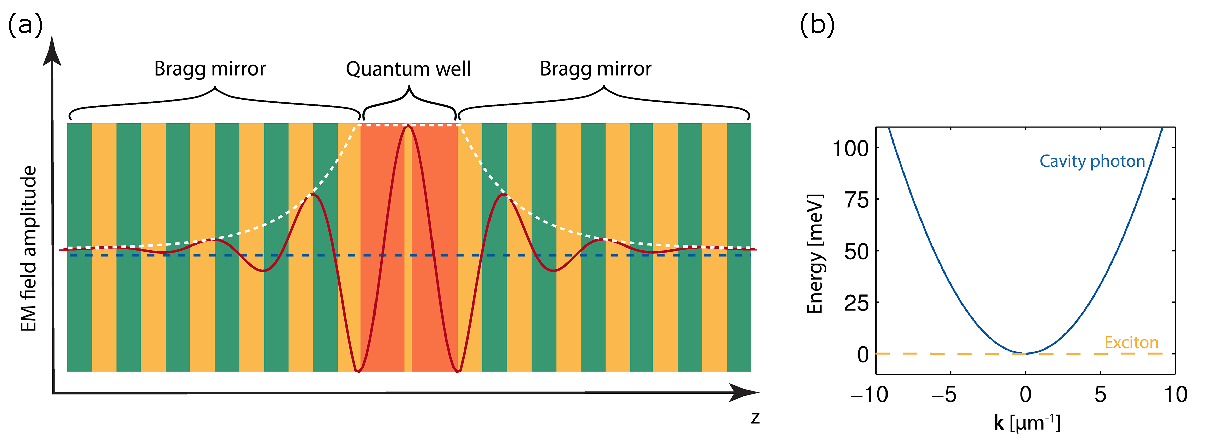
\includegraphics[width=0.8\linewidth]{chap_theory/fig/polariton_cavity.pdf}
    \caption{\textbf{Schematic representation of a quantum well embedded in an optical microcavity.} The quantum wells are placed at the antinode of the electric field of the cavity. The cavity is designed to have a single mode that matches the exciton energy.
    (b) Dispersions relation of the exciton (yellow) and photon (blue) modes in a typical microcavity. Since the exciton effective mass $m_X$ is $10^4$ times larger than the photon mass the exciton dispersion 
    looks flat with respect to the photon. The cavity has been designed so the $\kpar=0$ energies are matched.
    \label{fig:polariton_cavity}}
\end{figure}

The role of the latter is to create a set of resonant modes that will act as a "filter" for the exciton recombination. 
The quantization axis of the optical microcavity is chosen to be the same as the quantum well and the light-matter
interactions are optimized by placing the quantum well a the antinode of the electric field. The cavity length is chosen so that single photonic mode can be equal the excitonic energy.
This matching can be seen by looking simultaneously at the exciton and photon dispersion relation as a function of the in plane wavevector and check that they cross each other at a finite wavevector. For instance in the case of \autoref{fig:polariton_cavity} (b) the cavity has been designed so that the exciton and photon energies are equal at $\kpar=0$.
Several quantum well can then be stacked in the cavity to enhance the interactions provided that they are once again located at antinodes of the photonic field.
In the experiment we use a $3\lambda/2$ made of two planar DBR in which are placed three $InGaAs/GaAs$ quantum wells. An extended description of the fabrication procedure to built such a sample can be
found in \cite{maitre_thesis}. However, the main features mentionned so far can be summarized in a few points :

\begin{itemize}
    \item The cavity is made by embedding semiconducting quantum wells in between two distributed bragg reflectors forming a high finesse optical microcavity.
    \item The length of the cavity and of the wells are chosen so a single longitudinal mode of the electric field is resonant only with the 1s state of the exciton.
    \item The exciton are confined in the $xy$-plane in each quantum well and the exciton density can be tuned by changing the number of quantum wells.
    \item Momentum conservation still holds in the plane of the cavity. Namely, an incoming photon with wavevector $\kpar$ will create an exciton with the same in-plane wavevector. 
\end{itemize}
It appears then that the relevant motion of the interacting particles at stake lies in the $xy$-plane since the wavevectors in 
the  $z$-direction are fixed by the cavity parameters. Consequently, for sake of clarity, we will only refer to the in-plane wavevector in the following
by dropping the $\parallel$ label and just write $\kvec$.

\noindent Now that that some efforts were put in enhancing exciton-photon interactions let us see the different coupling regimes that we can be reached in such samples. 



\bigskip
\noindent \textbf{Coupling regimes.} At first approximation the problem can be thought as two bath of particles 
exchanging quanta at a rate $\OmR$. Depending on the efficiency of this exchage compared to
the damping rate of each bath $\gamma_X$ and $\gamma_{\gamma}$ one has to revisit the way to describe the system. Indeed, when 
$\OmR \ll \gamma_X, \gamma_{\gamma}$ the system is said to be in the weak coupling regime. It can be understood in terms of lifetimes : both excitons and photons lifetimes are too short compared to the 
characteristic time of the exchange $1/\OmR$. The energy leaks out of the system before it can change from one state to the other. The exciton-photon interaction is in this case irreversible.
If $\OmR \gg \gamma_X, \gamma_{\gamma}$ the system is said to be in the strong coupling regime. In a given photonic (or excitonic) lifetime $1/\gamma_{cav}$,
the answer to the question "where is the energy ?" is no longer clear. Indeed the energy have had enough time to coherently go back and forth between exciton and photon states plenty of times. Translating
this in quantum mechanics language simply means that the system is in a superposition of exciton and photon states. Polariton then rise in this regime as
as supersposition of microcavity photons and excitons exchanging energy at the so called Rabi frequency $\OmR$. 

\bigskip

\textbf{Linear Hamiltonian.} Let us write formally the coupling between excitons and photons described above. First we tackle
the weak optical excitation scheme in which non linear interactions among excitons can be neglected. The corresponding linear Hamiltonian 
is given by : 

\begin{equation}
    \Ham_{lin} = \sum_{\mathbf{k}}\left[E_X(\mathbf{k})b^{\dagger}_{\mathbf{k}}b_{\mathbf{k}} + E_{\gamma}(\mathbf{k})a^{\dagger}_{\mathbf{k}}a_{\mathbf{k}} + \dfrac{\hbar\OmR}{2}a^{\dagger}_{\mathbf{k}}b_{\mathbf{k}} + a_{\mathbf{k}}b^{\dagger}_{\mathbf{k}}\right]
    \label{eq:linear_hamiltonian}
\end{equation}
where $b^{\dagger}_{\mathbf{k}}$ and $a^{\dagger}_{\mathbf{k}}$ are the creation operators of the exciton and photon modes respectively. The first two terms account for the energies of the excitons and the photons while 
the terms $b^{\dagger}_{\mathbf{k}}a_{\mathbf{k}}$ and $a^{\dagger}_{\mathbf{k}}b_{\mathbf{k}}$ account for the linear exciton-photon coupling yielding an interaction energy $\hbar\OmR$. 
Obviously this hamiltionian is not diagonal in the excitons-photons operators basis.
Excitons-polaritons then arise as the two eigenstates of $\Ham_{lin}$ : the upper and the lower polaritons whose creation and annihilation operators are  $(\ukdag, \uk)$ and $(\pkdag, \pk)$ respectively.
These operators can be found by an unitary transormation on the exciton-photon basis that was extensively used by Hopfield \cite{hopfield_theory_1958}  :


\begin{equation}
    \label{eq:unitary_transformation}
    \begin{bmatrix}
    \pk \\
    \uk
    \end{bmatrix} 
    = 
    \begin{bmatrix}
    C_\kvec & X_\kvec \\
    X_\kvec & -C_\kvec
    \end{bmatrix}
    \begin{bmatrix}
    \ak \\
    \bk
    \end{bmatrix},
\end{equation}

where $C_\kvec$ and $X_\kvec$ are the Hopfield coefficients for photons and excitons respectively. The unitarity of the transformation
is reflected by the relation $C_\kvec^2 + X_\kvec^2 = 1$. As a consequence, they can be interpeted as the fractions of excitons and photons in both modes.
More precisely they depend on the excitons/photons energies and the Rabi frequency as : 

\begin{subequations}
    \begin{align}
    C_\kvec^2 &= \dfrac{\sqrt{\DeltaEX^2 + \hbar^2\OmR^2}- \DeltaEX}{2\sqrt{\DeltaEX^2 + \hbar^2\OmR^2}}, \\[5mm]
    X_\kvec^2 &=  \dfrac{\sqrt{\DeltaEX^2 + \hbar^2\OmR^2}+ \DeltaEX}{2\sqrt{\DeltaEX^2 + \hbar^2\OmR^2}}.
    \end{align}
    \label{eq:hopfield_coefficients}
\end{subequations}
where $\DeltaEX(\kvec) = E_{\gamma}(\kvec)-E_X(\kvec)$ is the detuning between the exciton and the photon energies at $\kvec$. 
In this basis the linear hamiltonian can be written in its diagonal form.



\begin{equation}
    \Ham_{lin} = \sum_{\mathbf{k}}\left[E_{LP}(\mathbf{k})\ukdag\uk + E_{UP}(\mathbf{k})\pkdag\pk\right]
    \label{eq:linear_hamiltonian_diagonal}
\end{equation}
where the eigenvalues $E_{LP}(\mathbf{k})$ and $E_{UP}(\mathbf{k})$ are the lower and upper polariton dispersion relation. Their analytical expressions 
are given by :

\begin{equation}
    \begin{align}
    E_{LP}(\mathbf{k}) &= \dfrac{E_X(\mathbf{k})+E_{\gamma}(\mathbf{k})}{2} - \dfrac{\sqrt{\DeltaEX^2 + \hbar^2\OmR^2}}{2}, \\[5mm]
    E_{UP}(\mathbf{k}) &= \dfrac{E_X(\mathbf{k})+E_{\gamma}(\mathbf{k})}{2} + \dfrac{\sqrt{\DeltaEX^2 + \hbar^2\OmR^2}}{2}.
    \end{align}
    \label{eq:polariton_dispersion}
\end{equation}

\textbf{Tuning the exciton-photon fraction.} As it can be seen the weight of photon and exciton in a given polaritonic state can be then tuned by changing the exciton-photon detuning 
$\DeltaEX$. Particurlarly, when $\DeltaEX = 0$ we have $C_\kvec^2= X_\kvec^2 = \frac{1}{2}$ meaning that the exciton and the photon are equally mixed in the polariton states. In practice, there are two ways to change the exciton-photon detuning. The first tuning knob, which is the most obvious, is the wavevector $\kvec$. Since the exciton
dispersion is flat with respect to the photon it boils down to move on the photon dispersion curve. Still, exciting a polariton state with a given set of Hopfield coefficients will fix the wavevector and, in some case might not be even possible. 
For instance if the photonic dispersion is above the exciton energy at all wavevector as in   \autoref{fig:wedge_and_hopfields} $\mathrm{b_1)}$, it is impossible to reach the purely hybrid configuration $\DeltaEX = 0 $. Creating an arbitrary polaritonic state thus require a second knob to tune $\DeltaEX$. It is generally done by introducing a small wedge between the two DBR that will change the photon resonance condition as shown in \autoref{fig:wedge_and_hopfields} a) : a change in the cavity length $L$ will shift vertically the photon disperions.
 Luckyly, this comes for free with the usual Molecular Beam Epitaxy method used to grow the sample.
The principle is to heat the target material to its sublimation temperature to produce a molecular beam that is then deposited on a substrate to form thin atomic layers that stack on top of each other.
In practice, the substrate is located on a spinning disk to avoid the molecule to clusterise. If the spinning disk is stopped, molecules will accumulate in the center of the beam and form a "hill".
By taking advantages of this features it is possible to change progressively the thickness of the layer and thus the cavity resonance condition. A given sample
has in fact a wide range of exciton-photon detuning that can be adressed in the lab by changing the working point on the cavity. 

\begin{figure}[]
    \centering
    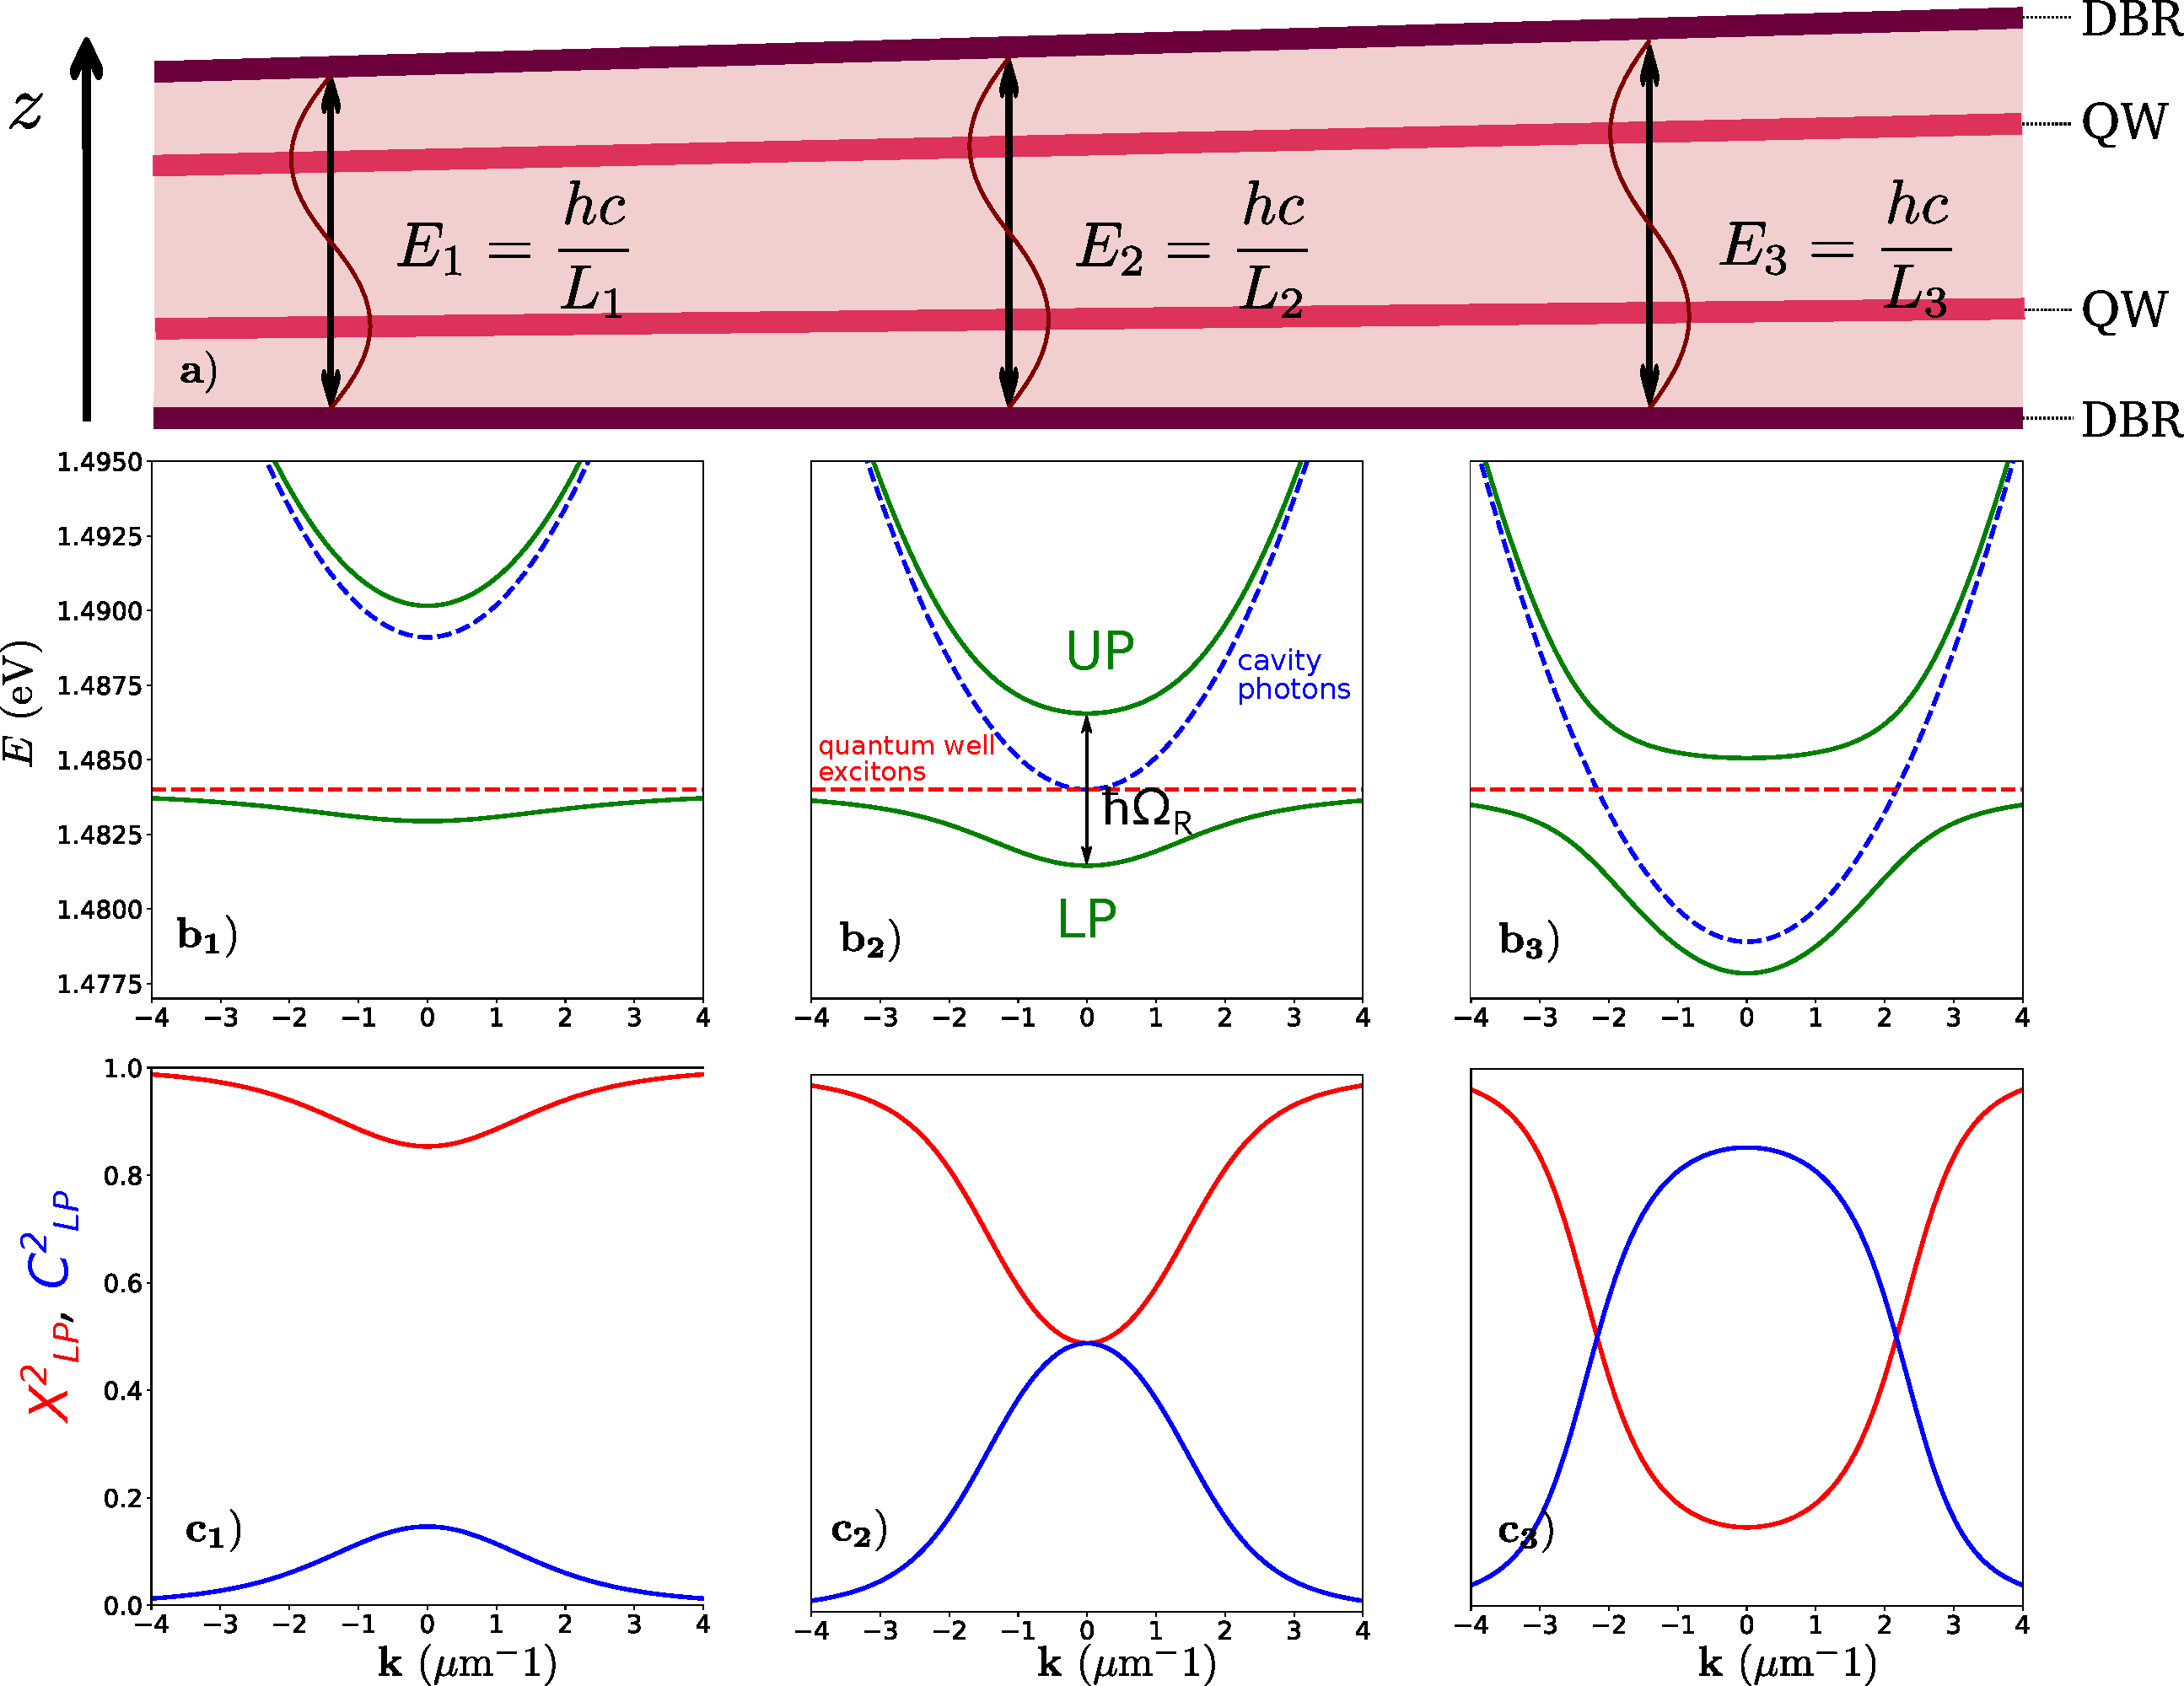
\includegraphics[width=1\linewidth]{chap_theory/fig/wedge_and_hopfields.pdf}
    \caption{\textbf{Scheme of an optical microcavity with a wedge, polaritons dispersion relations and Hopfield coefficients.} \textbf{a)} Side view of a
    double quantum well semiconducting microcavity. From left to right the photon resonant energy decreases as the length of the cavity increases. The exciton energy remains constant since it is fixed by the width of the quantum well.
    We take as example three point in the sample $i=1,2,3$ with increasing cavity length. At each point the wavy lines represent the optical standing wave stemming from the resonance conditions $\lambda_i = L_i$
    The corresponding energies $E_i$ illustrate the three different regimes namely : $\DeltaEX^{(1)}(\kvec=0) >0 , \DeltaEX^{(2)}(\kvec=0)=0 , \DeltaEX^{(3)}(\kvec=0) <0 $. Each $E_i$ corresponds to the subplots
    $\mathrm{b_i)}$ and $\mathrm{c_i)}$. $\mathbf{b_1), b_2), b_3)}$ Dispersion relations of the lower (LP) and upper polaritons (UP) in a typical microcavity for each value of $\DeltaEX^{(i)}$. The exciton energy is the yellow dashed line while the photon energy is the blue dashed line. Depending on the location
    on the sample $i=1,2,3$ the photon dispersion curve gets shifted vertically yielding different values of the Hopfield coefficient. $\mathbf{c_1), c_2), c_3)}$ Corresponding Hopfield coefficients as a function of the in-plane wavevector for the three different regimes. Adapted from \cite{claude_phd}.
    \label{fig:wedge_and_hopfields}}
\end{figure}

In general, when the exciton-photon detuning is too positive the UP branch recovers the excitons curve while the LP branch recovers the photons curve. Conversely,
when the exciton-photon detuning is negative the UP branch recovers the photons curve while the LP branch recovers the excitons curve. This is not very suprising
since a great detuning means that the exciton and the photon are far from each other making the coupling less efficient.  At the zero detuning point 
$\DeltaEX=0$ the coupling is maximum and the splitting between the lower and upper polariton branch is equal to the Rabi energy frequency $\hbar\OmR$. Besides, the anticrossing
between the two branches is a direct consequence of the strong coupling regime and can be find even in classical systems like coupled pendulums. 

The suitable range of detuning for which the polariton concept is still relevant and that we can adress in the experiment is shown in \autoref{fig:anticrossing}
\bigskip

\textbf{Relaxation.} The strong coupling condition $\OmR \gg \gamma_X, \gamma_{cav}$ can also be seen by directly taking into account
the finite lifetime of excitons and photons, introducing imaginary energies $E_{\gamma}-i \gamma_{cav}$ and $E_X-i\gamma_X$ as in \cite{cohen-tannoudji_photons_2004}.
Doing so, the polariton dispersions relation become :

\begin{align}
    \begin{split}
        E_{UP, LP}(\kvec) ={}& \dfrac{\Eph(\kvec) + \Eex(\kvec)}{2} - i \hbar \dfrac{\gamma_{cav} + \gamma_X}{2}
        \\& \pm \dfrac{1}{2} \sqrt{\left[ \hbar \OmR \right]^2 + \left[ \DeltaEX - i \hbar (\gamma_{cav} -  \gamma_X )\right]^2}.
    \end{split}
    \label{polariton_disp_loss}
    \end{align}
At zero detuning we obtain :

\begin{equation}
        E_{UP, LP}(\kvec) =\Eex(\kvec) - i \hbar \dfrac{\gamma_{cav} + \gamma_X}{2} \pm \dfrac{1}{2} \sqrt{(\hbar \OmR) ^2 +  (\hbar\gamma_{cav} - \hbar \gamma_X )^2}.
    \label{polariton_disp_loss_zero_det}
\end{equation}
The existence of two distinct energies for the two polaritons modes thus depends on the relative values of $\OmR$ and $|\gamma_{cav} - \gamma_X|$.
 If the coupling constant $\OmR$ is smaller than the difference between the relaxation constants, the two eigenenergies share the same real part, and the degeneracy between the exciton and the cavity mode remains unbroken.
Being a supersposition of excitons and photons the polaritons also have a relaxation rate that can then be inferred from the imaginary part of their energy :

\begin{subequations}
    \begin{align}
    \gamma_{UP}(\kvec)&= X_\kvec^2\gamma_{cav} + C_\kvec^2\gamma_X, \\[5mm]
    \gamma_{LP}(\kvec)&= X_\kvec^2\gamma_X + C_\kvec^2\gamma_{cav}.
    \end{align}
    \label{eq:polariton_relaxation}
\end{subequations}
Once again, the hopfield coefficient have a strong impact on the polariton relaxation rate. In the range of detuning
available in our sample we measure relaxation rates of the order of  $\SI{70}{\micro\electronvolt}$ which correspond to a lifetime  
$\tau \sim \SI{10}{\pico\second}$. This value is beyond the time response of a wide class of instruments and require generally both pulsed lasers and ultrafast
detection devices to be resolved as in \cite{Utsunomiya_fluidlightexp_2008}. The present work is not dedicated to time resolved experiments as we rather use a continuous wave laser to constantly compensate for the losses and reach a steady state from which we extract observable quantities. This system is then highly out of
equilibrium. Although this feature seems limiting at first sight it can actually turn into an asset whenever one wants to study dynamical instabilities. Indeed, in conservative systems, 
instabilities are difficult to study precisely because they tend to make the system unstable. In the case of polaritons, the losses can reduce 
their effect while keeping their signature visible in the steady state of the system \cite{claude_high-resolution_2022}.

\bigskip


\textbf{Effective mass.} By analogy with was done for the photons in \autoref{sec:photon} it is possible to affiliate an effective mass to the polaritons
by taking the second derivative at the bottom of the polariton dispersion relation, namely :

\begin{subequations}
    \begin{align}
    \dfrac{1}{m_{UP}} &= \dfrac{X_0^2}{m_X}+\dfrac{C_0^2}{m_{\gamma}}, \\
    \dfrac{1}{m_{LP}} &= \dfrac{X_0^2}{m_{\gamma}}+\dfrac{C_0^2}{m_X}.
    \end{align}
\end{subequations}
Reminding that $C_0^2 + X_0^2 = 1$ and that $\frac{m_\gamma}{m_X}\ll 1$. It can be cast in the following form :

\begin{subequations}
    \begin{align}
    m_{UP} &\approx\dfrac{m_\gamma}{X_0^2} \\
    m_{LP} &\approx\dfrac{m_X}{C_0^2}
    \end{align}
    \label{eq:polariton_effective_mass}
\end{subequations}
It can be seen that polaritons inherit the low effective mass of the photons making their transport easier than for excitons.
This is particularly interesting for the realisation of polaritonic circuits in the framework of quantum information processing \cite{liew_optical_circuit_2008}.
The excitonic part of the polariton also bring its own features to the table. In particular, the strong exciton-exciton non linear interactions that
will turn light into a fluid of interacting particles. This is the subject of the next section.
\begin{figure}[h]
    \centering
    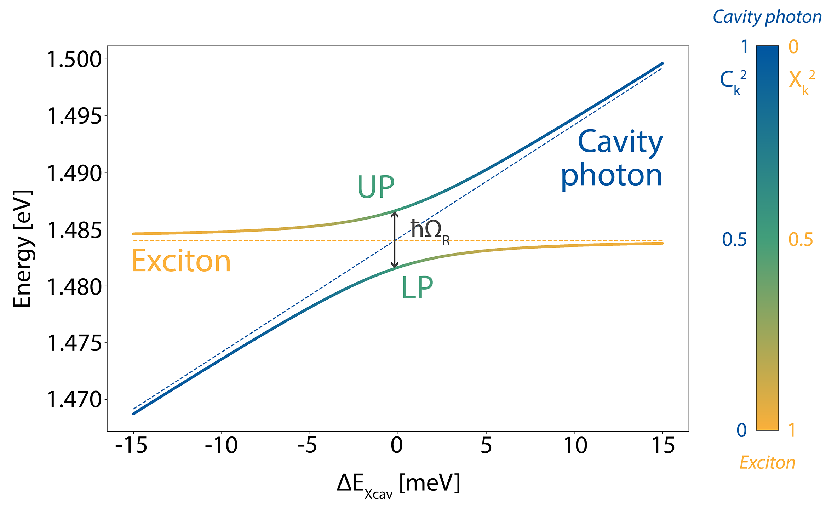
\includegraphics[width=0.75\linewidth]{chap_theory/fig/anticrossing.pdf}
    \caption{\textbf{Anticrossing in the strong coupling regime.} Energies of the upper (UP) and lower (LP) polariton branches at $\kvec = 0 \mathrm{\mu m^{-1}}$, with respect to the exciton-photon detuning at zero wavevector $\DeltaEX(\kvec=0)$ and the color-coded squared modulus of the Hopfield coefficient $X^2$ (exciton) and $C^2$ (photon). The yellow and blue dashed lines are respectively the bare exciton and photon energies. 
    At $\DeltaEX$ = 0 meV, the coupling is the better yielding an energy splitting equal to the Rabi energy $\hbar \OmR$. Adapted from \cite{maitre_thesis}}. 
    \label{fig:anticrossing}
\end{figure}

\subsection{Polariton interactions}
\label{sub:polariton_interactions}

It is now clear that shinning a strong laser with the right frequency on a semiconducting microcavity will create plenty of polaritons. Since the have an excitonic part,
they may undergo many body effects that were not taken into account in the linear hamiltonian model derived earlier. More precisely, polaritons experience 
all the exciton-exciton interactions described in \autoref{sub:exciton_exciton_interaction} as well as additional features coming from their coupling with light.
Remarkably, in high density regime the Pauli principle has to apply again on the electrons and the holes leading to carrier exchanges. In the absence of light
these fermionic exchanges are actually the dominant scatterings processes while the direct Coulomb scattering is negligible as was explained in \autoref{sub:exciton_exciton_interaction}.
We remind the expression of the resulting exchange hamiltonian :

\begin{equation}
    \Ham_{XX} = \dfrac{1}{2}\sum_{\mathbf{k}, \mathbf{k}', \mathbf{q}}V_{XX}\left[p^{\dagger}_{\mathbf{k+q}}p^{\dagger}_{\mathbf{k'-q}}p_{\mathbf{k}}p_{\mathbf{k'}}\right]
    \label{eq:direct_pol_interaction}
\end{equation}

When the excitons are strongly coupled to cavity photon these carrier exchanges give rise to an additional saturation potential describing what was called a "photon-assisted exchange scattering" in the proposal of \cite{Combescot_2007_exact_pol_pol_interactions}.:


\begin{equation}
    \Ham_{sat} = \dfrac{1}{2} \sum_{\kvec, \kvec', \mathbf{q}} V_{sat} \left[ a^\dagger_{\kvec+ \mathbf{q}} b^\dagger_{\kvec'- \mathbf{q}} b_{\kvec} b_{\kvec'} + h.c. \right],
\end{equation}
where $V_{sat}$ is the saturation potential that can be computed by applying the Usui transformation on the quantum wells \cite{usui_sat_potential_1960}.

\begin{equation}
    V_{sat}=\dfrac{\hbar\OmR}{An_{sat}},
\end{equation}

in which $n_{sat}$ is the saturatiion density computed from the 2D exciton bohr radius as $n_{sat}=1/a_X^{QW}$ and A the macroscopic quantization area.
\textcolor{red}{This scattering can be understood from a microscopic point of view. Consider two excitons, $i_1$ and $i_2$, in a first step they exchange their carrier without any Coulomb process giving
two other excitons $i_1'$ and $i_2'$. In a second step, one of the exciton, let us say $i_1'$ find itslef in the same state than a neighbouring exciton. Because of the Pauli principle it can not stay in this state. Luckyly it is couple 
to cavity photon which enable it to get out of this irregular situation by emitting a photon.}
To end up with a description of interactions in the polariton basis we invert the unitary transformation in \autoref{eq:unitary_transformation} : 

\begin{subequations}
    \begin{align}
        \bk &=X_k \pk -C_k\uk, \\
        \ak &=C_k \pk +X_k\uk,
    \end{align}
\end{subequations}
and inject these expressions into $\Ham_{XX}$ and $\Ham_{sat}$. We end up with a single polariton-polariton potential that is a combination of hopfield coefficients, $V_{sat}$ and $V_{XX}$.
For the lower polaritons, which are the one we excite in the experiment and to which we will restrict in the following we obtain an effective polariton-polariton potential $V_{pp}$ as :

\begin{equation}
    V_{pp}= |X_\kvec|^4V_{XX}+2|X_\kvec|^2X_\kvec C_\kvec V_{sat}.-
\end{equation}
Once again it depends on the exciton-photon fraction through the Hopfield coefficients, and, in the purely hybrid situation $\DeltaEX$=0, yields $A \times V_{pp}= \SI{1}{\micro\electronvolt \per\square\micro\meter}$ in our sample.

\bigskip

\textbf{Non linear LP hamiltonian.} Finally, taking into account the polariton-polariton interactions abovementionned the linear hamiltonian for Lower Polaritons can be completed as follows :

\begin{equation}
    \Ham_{LP} = \sum_{\mathbf{k}}\hbar\omega_{LP}(\mathbf{k})\pkdag\pk + \dfrac{1}{2}\sum_{\kvec,\kvec',\mathbf{q}}V_{pp}\left[p_{\kvec+ \mathbf{q}}^{\dagger}p_{\kvec'- \mathbf{q}}^{\dagger}p_{\kvec}p_{\kvec'}\right].
    \label{eq:pol_non_linear_hamiltonian}
\end{equation}

\textbf{Energy renormalization.} As it can already be seen in the LP non linear hamiltonian, the bare polartion energies are no longer eigenvalues of the system in the presence of interactions.
To give a simple picture of this feature let us restrict the description to two polariton modes $p_{\mathbf{k_1}}$ and $p_{\mathbf{k_2}}$.
If the system is prepapred in such a way as to populate one of the two modes, $\mathbf{k_2}$, this macroscopic reservoir of polaritons acts as an external potential for the polaritons in the poorly populated mode $\mathbf{k_1}$. Consequently, the energy of the polaritons in mode $\mathbf{k_1}$ increases by an amount corresponding to the potential created by the polaritons in mode $\mathbf{k_2}$. 
This is a phenomenon of energy renormalization.

To be more quantitative, we can write the Hamiltonian of the system while restricting it to these two modes. In this case, $\Ham_{int}$ is the sum of $p^\dagger_\mathbf{k_1}p^\dagger_\mathbf{k_2}p_\mathbf{k_1}p_\mathbf{k_2}$ and $p^\dagger_\mathbf{k_2}p^\dagger_\mathbf{k_1}p_\mathbf{k_2}p_\mathbf{k_1}$. Since $p_\mathbf{k_2}$ and $p_\mathbf{k_1}$ are eigenstates of the system, they commute, meaning that the two previous term account for the same scattering.
The time evolution of $p_{\mathbf{k_1}}$ can then be described by the Heisenberg equation : 

\begin{equation}
    i\hbar \dfrac{d}{dt}p_\mathbf{k_1} = [p_\mathbf{k_1}, \Ham_{LP}] = [p_\mathbf{k_1},\Ham_{lin}] + [p_\mathbf{k_1},\Ham_{int}].
\end{equation}

the interacting term being :

\begin{equation}
    [p_\mathbf{k_1},\Ham_{int}]=\dfrac{V_{pp}}{2}p^\dagger_\mathbf{k_2}p^\dagger_\mathbf{k_2}p_\mathbf{k_1}= \dfrac{\hbar g_{LP}}{A}\hat{N}_{2}p_\mathbf{k_1}.
\end{equation}
$\hat{N}_{2}$ is the number operator in mode $\mathbf{k_2}$ and $\hbar g_{LP} = V_{pp}A/2$  is the polariton-polariton interaction constant. Since, the mode 
$\mathbf{k_2}$ is macroscopically populated, we can replace $\hat{N}_{2}$ by its expectation value $\langle \hat{N}_{2} \rangle$, which exhibit the polariton density in mode $\mathbf{k_2}$, $n_{2}=\langle \hat{N}_{2} \rangle/A$.
As a result, the master equation for the $\kvec_1$ gets renormalized by interactions with the $\kvec_2$ mode as :

\begin{equation}
    i\hbar \dfrac{d}{dt}p_\mathbf{k_1} = \left[\hbar\omega_{LP}(\mathbf{k_1}) + \hbar g_{LP}n_{2}\right]p_\mathbf{k_1}.
    \label{eq:renormalized_energy}
\end{equation}
where $\omega_{LP}(\mathbf{k_1})=E_{LP}(\kvec_1)$ is the bare energy of the polariton with wavevector $\kvec_1$. Although this is a simplified model with only two modes, the equation demonstrates how interactions between polaritons can lead to the renormalization of their energies. More generally, this phenomenon takes place between all modes in the system, including self-interactions of individual modes.
 The latter closely resembles the optical Kerr effect, where a field modifies the refractive index of the medium through which it propagates.

\section{Polariton dynamics}

\indent 

To summarize, microcavity exciton-polaritons are hybrid light-matter quasiparticles that combine characteristics of both components. 
Their photonic part endows them with an exceptionally low effective mass and allows us to manipulate them using light. 
Conversely, their excitonic part provides them with the exotic properties associated with electrons in semiconductors. 
Although the resulting interactions are varied and stem from different origins, they can, to a first approximation, be described by a single four-body contact potential, $V_{pp}$.

In this framework, polaritons can be viewed as weakly interacting bosons, distinguished by their inherent losses, making their behavior an out-of-equilibrium problem. 
In the following, we will explore their dynamics when one or a few modes are macroscopically populated, revealing remarkable phenomena typically associated with true many-body bosonic systems, such as superfluidity and Bose-Einstein condensation (BEC).
 However, whenever necessary, we will return to their composite fermionic nature to account for unique features that may not be captured by the mean field approximation.
 
\subsection{Mean field approximation}

\indent

In order to describe the dynamics of the polariton fluid of light, it is convenient to use the mean field approximation as it is usually done for quantum fluids \cite{pitaevskij_bose-einstein_2016}. This assumption is valid when the number of particles is large $N \sim N+1$ and when the major part of them occupy the same quantum state.
Obviously, the latter can happen only in bosonic systems since fermions obey the Pauli exclusion principle. In atomic systems, the macroscopic occupation occurs in the ground state of the system, and, provided that the temperature is low enough, happens spontaneously due to bosonic stimulation. In the case of polaritons, the situation is dramatically different since the system is out of equilibrium and the particles have to be continuously pumped to compensate for the losses.
The mean field of the system is then rather a steady state than a ground state at equilibrium. This being said, it is still possible to define a macroscopic occupation of a given mode in the system.
Whenever this happens, the theoretical procedure boils down to replacing the field operator $\hat{\psi}(\mathbf{r},t)= \sum_{k}\varphi_\kvec \hat{p}_\kvec$ that annihilates a particle at ($\mathbf{r}$,t), by its expectation value $\langle \hat{\psi}(\mathbf{r},t)\rangle$. This idea is supported by
by the fact that, in such situations, adding or removing a particle from the system does not change its state. The system is then described by a single classical wavefunction whose square modulus gives the density of particles in the system $|\psi(\mathbf{r},t)|^2= n(\mathbf{r},t)$ and with a well defined phase 
accounting for long range coherence. However, it doesn't mean that the system has became fully classical. Indeed, its quantum nature is hidden in the fluctuations around the mean field and often manifest itself through collective behavior. Accounting for these fluctuations is done 
by adding a small perturbation to the mean field : 

\begin{equation}
    \label{eq:mean_field_and_fluctuation}
    \hat{\psi}(\mathbf{r},t) = \langle \psi(\mathbf{r},t) \rangle + \delta \psi(\mathbf{r},t).
\end{equation}

For now let us focus on the description of the mean field dynamics and justify more quantitavely the relevance of describing a polariton fluid with a single wavefunction.

\bigskip

\textbf{One wavefunction to rule them all.} A pioneering result in the early stages of quantum mechanics is the so called wave-particle duality proposed by Louis de Broglie \cite{deBroglie1925} in 1924.
It states that particles can exhibit both wave and particle properties. 
More precisely, to any particle with momentum $\mathbf{p}$ can be associated a wavelength $\lambda=h/|\mathbf{p}|$. This wavelength is the characteristic of the wave associated with the particle and is called the de Broglie wavelength. 
As a result if two particle are separated by a distance smaller than their de Broglie wavelength their corresponding wavefunction will sum and possibly give rise to wave like effect as interferences.
This idea was later confirmed by the famous double slit experiment in which electrons were sent through a double slit and displayed an interference pattern.

If one apply this idea to a great number of particle in the same quantum states whose inter-particle distance is smaller than $\lambda$ it is no longer possible to distinguish them and they can be described by a single wavefunction.
At thermal equilibrium the momentum of a particle follows a Maxwell Boltzmann distribution and the de Broglie wavelength is of the order of the thermal de Broglie wavelength :
\begin{equation}
    \lambda_T = \dfrac{h}{\sqrt{2\pi m k_B T}},
    \label{eq:thermal_deBroglie}
\end{equation}
where $T$ is the temperature $m$ the particle mass and $k_B$ the Boltzmann constant. From this simple formula, one can see why reaching long range coherence in a system often require trapping and cooling procedures. In the case of polaritons,
a typical polariton-polariton inter-distance is about $\SI{0,1}{\micro\meter}$ while the small polaritons effective mass and the cryogenic temperature ($\sim 4K$) yields a thermal de Broglie wavelength of the order of $\SI{1}{\micro\meter}$ which validates the mean field approximation.
Now that we have a single order parameter to describe the system, let us see how it evolves in time.

\bigskip

\subsection{Driven dissipative Gross-Pitaevskii Equation.}
In the context of Bose gas this problem was first tackled by Gross \cite{Gross1961} and Pitaevskii \cite{pitaevskii1961} to describe
the structure of quantized vortices in liquid Helium. The resulting equation is known as the \textit{Gross-Pitaevskii equation} or non-linear Schrödinger equation :

\begin{equation}
     i\hbar \dfrac{\partial}{\partial t} \psi(\rvec, t) = \left( -\dfrac{\hbar^2}{2 m}\nabla_\rvec^2 + V_{ext}(\rvec) + \hbar g \abs{\psi(\rvec, t)}^2 \right) \psi(\rvec, t),
\label{GPE}
\end{equation}
where $g$ is the interaction constant, $\nabla_\rvec$ the kinetic energy and $V_{ext}(\rvec)$ is the external potential experienced by the particles. To extend this equation to the out of equilibrium polariton case, a first formulation in 
terms of exciton and photon reveals to be enlightening to identify the various corrections that must be considered.
Losses are incorportated through the relaxation rates $\gamma_X$ and $\gamma_{cav}$ while the continuous injection of photons in the system is accounted for by a pumping term $F_p(\rvec,t)$ in the photon field master equation.
Considering these terms we end up with a set of coupled equation for the exciton and photon fields $\psi_X(\rvec,t)$, $\psi_{\gamma}(\rvec,t)$ :

\begin{equation}
    i\hbar \dfrac{d}{dt}
    \begin{bmatrix}
    \psi_{\gamma}(\rvec, t) \\
    \psi_{X}(\rvec, t)
    \end{bmatrix} 
    = 
    \begin{bmatrix}
    \hbar F_p(\rvec, t) \\
    0
    \end{bmatrix} +
\label{Schrödinger_uncoupled}
\end{equation}
\begin{align*}
    \left( \Ham_{lin}(\rvec) + 
    \begin{bmatrix}
    V_\gamma(\rvec) - i\hbar \dfrac{\gamma_{cav}}{2} & 0\\
    0 & V_X(\rvec) - i\hbar \dfrac{\gamma_{X}}{2} + \hbar g_{XX} n_{X}(\rvec, t)
    \end{bmatrix}
    \right)
    \begin{bmatrix}
    \psi_{\gamma}(\rvec, t) \\
    \psi_{X}(\rvec, t)
    \end{bmatrix},
\end{align*}    
where $V_\gamma(\rvec)$ and $V_X(\rvec)$ are the mean external potentials felt by photons and excitons respectively, $g_{XX} = A V_{XX}/2\hbar$ is the exciton interaction strength and $n_X = \abs{\psi_{X}}^2$ is the exciton density.  Additionally, $\Ham_{lin}(\rvec)$ corresponds to the linear Hamiltonian from \autoref{eq:linear_hamiltonian_diagonal}, expressed in real space by substituting $\kvec$ with $i \nabla_\rvec$.

\begin{equation}
    \Ham_{lin}(\rvec)
    = 
    \begin{bmatrix}
    \hbar \omega_X & \hbar \OmR / 2 \\
    \hbar \OmR / 2 & \hbar \omega_\gamma(-i \nabla_\rvec)  
    \end{bmatrix}.
\end{equation}
as explained earlier, the exciton dispersion relation can be safely considered constant with respect to the photon one, $\hbar \omega_X(\kvec)=\hbar \omega_X(0)$.
We can then transition to the polariton basis, obtaining two decoupled equations for the lower and upper polariton fields, $\psi_{LP}(\rvec,t)$ and $\psi_{UP}(\rvec,t)$. Focusing on the lower polariton branch, this leads to the so-called \textit{driven-dissipative Gross-Pitaevskii equation}:
\begin{equation}
    \begin{align}
    i \hbar \dfrac{\partial}{\partial t} \psilp(\rvec, t) &= \left[ \hbar \omlp^0 -\dfrac{\hbar^2}{2 \mlp}\nabla_\rvec^2 + V_{LP}(\rvec) + \hbar g n(\rvec, t) - i \hbar \dfrac{\gamlp}{2} \right] \psilp(\rvec, t) + \hbar \eta_{LP} F_p(\rvec, t) \\
        &\coloneq \Ham_{LP} \psilp(\rvec, t) + \hbar \eta_{LP} F_p(\rvec, t),
    \end{align}
    \label{eq:generalized_GPE}
\end{equation}
where $V_{LP}$ is the external potential experienced by the polaritons which depend on those felt by photons and excitons through the Hopfield 
coefficients $V_{LP}(\rvec) = C^2_\kvec V_{\gamma} + X^2_\kvec V_{X}$, $\kvec$ being here the pump wavevector. The term $\hbar \omlp^0$ is the polaritons energy at zero wavevector while the $\hbar^2\nabla^2_\rvec /2\mlp$ is again the kinetic energy. Finally, the prefactor $\eta_{LP}$ account for the coupling efficiency of the pump photons whithin the system.
Since the presence of a fluid in the sample change the optical resonance through non linear interaction this term is generally not constant. However, in first approximation it is linked the reflectivity of the sample front mirror and can be considered as a constant. A full derivation of this equation as well as a complete discussion on its validity can be found in \cite{carusotto_quantum_2013}.

\bigskip


\textbf{Dark reservoir. }Along our description of excitons we mentionned the presence of dark excitons that are not directly coupled to light because of spin selection rules. As a consequence, one could think 
that they are not involved in the polariton dynamics. It is actually not the case. Indeed, eventhough they do not interact with photons they can still interact with bright excitons through the many complex electron-hole interactions described in \autoref{sub:exciton_exciton_interaction}.
Forgetting them in the description of the polariton dynamics would then be a mistake \cite{Menard2014, stepanov_dispersion_2019}. To derive a single master equation starting from the many microscopic interactions between photons, dark and bright excitons would require a full spin resolved description and is beyond the scope of this manuscript.
Nevertheless, we will account for their presence phenomenologically by considering them as a reservoir of density $n_r$ coupled to polaritons through a relaxation term $\gamma_{r}$. In terms of equations it reads as :


\begin{align}
    \begin{split}
        i \hbar \dfrac{\partial}{\partial t} \psilp(\rvec, t) ={}& \left[ \hbar \omlp^0 -\dfrac{\hbar^2}{2 \mlp}\nabla_\rvec^2 + V_{LP}(\rvec) + \hbar g n(\rvec, t) + \hbar \gr \nr(\rvec, t) - i \hbar \dfrac{\gamlp + \gamin}{2} \right] \psilp(\rvec, t)  \\&+ \hbar \eta_{LP} F_p(\rvec, t),
    \end{split}
    \end{align}
    
    \begin{equation}
         \dfrac{\partial}{\partial t} \nr = -\gamr \nr + \gamin n.
         \label{reservoir_eq}
    \end{equation}

As it will be shown in the following the presence of a dark reservoir is of great importance when it comes to describing the quantum fluctuations of the polariton fluid.


\subsection{Excitation scheme} So far, the derivation of the master equation was initiated by stating that a polaritonic state could be macroscopically populated 
through optical pumping. However, the pump term was not yet defined in the sense that we did not specify the frequency of the pump photons with respect to the polariton dispersion relation.
The latter is crucial to determine what are the mechanism leading to long range coherence. 

\bigskip

\subsubsection{Off resonance excitation} In the case off resonant case the pump laser is highly blue detuned with respect to the polariton energy, close to a reflecitivity minimum above the stop band of the DBRs (see \autoref{fig:DBR}).
The rise of a macroscopic population then occurs in the botom of the LP branch through polaritons relaxation. More precisely, the injected photons create highly excited electron-hole pairs that relax through the emission of phonons. 
Lowering their energy they can emit photons and, at some point, eventually strongly couple to them to form polaritons. At this stage the polaritons are incoherent since the coherence of the pump laser got lost in the many relaxation processes.
Then, the incoherent polariton undergo scatterings and relax toward the minimum energy states available. If the pump intensity is increased, the population in the minimum of the LP branch will "accelerate" the relaxation of the other polaritons through bosonic stimulations.
If the stimulation is efficient enough with respect to the losses, the bottom of the LP branch gets macroscopically populated and obtain a long range order which can be seen on \autoref{fig:polariton_bec}. Just like in atomic systems, the phase of the condensate wave function is chosen randomly through $U(1)$ symmetry breaking and is not inherited from the pump laser.
Such a phase transition in polariton planar microcavity was first observed in 2006 by Kasprzak et al. \cite{kasprzak_boseeinstein_2006}. 


Some major differences with atomic BECs are worth mentioning. First, the temporal phase of an atomic BEC is defined by the chemical potential and is related to the number of atoms in the system while 
the polaritonic system can never reach equilibrium. Its temporal phase result from a complex interplay between the pump laser and the losses of the system : the phase transition is driven by the pump intensity rather than the temperature.
transverse

\begin{figure}[H]
    \centering
    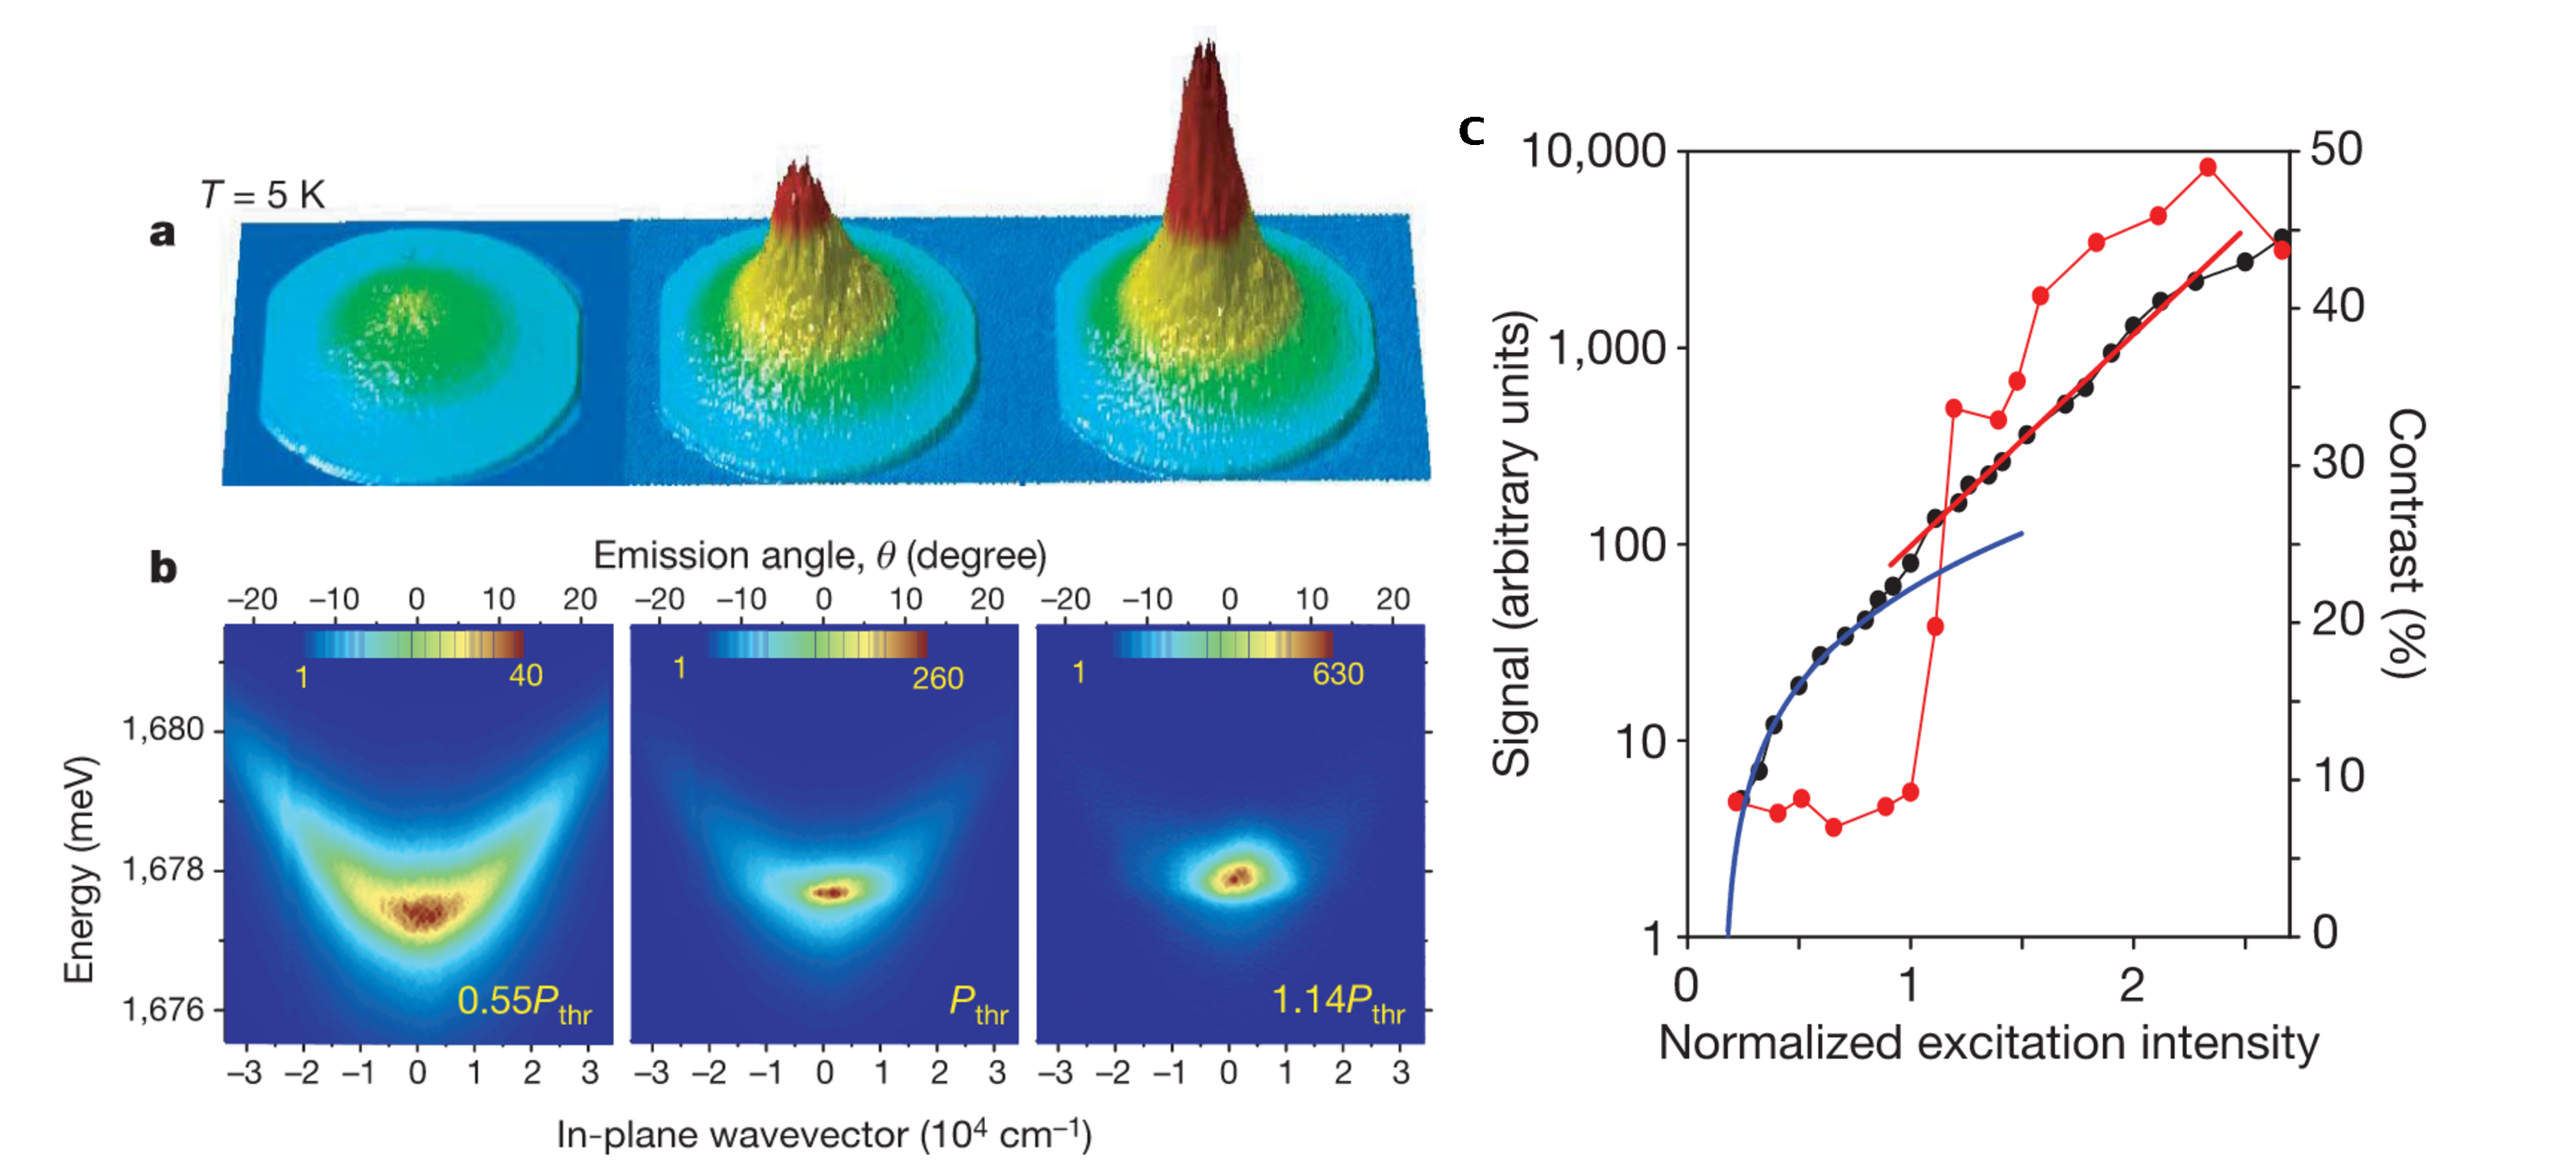
\includegraphics[width=1\linewidth]{chap_theory/fig/polariton_bec.pdf}
    \caption{\textbf{Bose-Einstein condensation of polaritons.} \textbf{a)} Far field emission of the fluid for increasing pump intensity. Above threshold, a strong emission in the zero wavevecotr mode is observed. \textbf{b)} Polariton dispersion for increasing pump intensities. Above threshold the bottom of the LP branch is macroscopically populated.
     \textbf{c)} Spatial correlation measurements using a Michelson interferometer.Solid red circles indicate correlations between two spots separated by 6mm (2.5 times the thermal de Broglie wavelength) within the condensate as a function of the excitation power. The correlation exhibits a threshold-like behaviour. 
     The variation of the ground-state emission intensity, normalized to the excitation power, is shown for comparison (solid black circles). The solid blue line is a quadratic fit of the data demonstrating the occurrence of particle-particle interaction below threshold. Above threshold, the solid red line is an exponential fit demonstrating the strong stimulation of the relaxation by the high occupancy factor of the ground state.Adapted from \cite{kasprzak_boseeinstein_2006}.}
    \label{fig:polariton_bec}
\end{figure}


\bigskip

\subsubsection{Resonant excitation.} In the resonant case, the pump laser is tuned near the polariton energy. The population of the polaritons is then directly driven by the pump laser. In particular due to momentum and energy conservation, the spatial and temporal coherence of the pump laser are transfered to the polaritons fluid. 
In that case the phase of the fluid is fixed by the pump and therefore is not randomly chosen. In this excitation scheme the fluid should then not be called a condensate. However, it can still exhibit superfluidity and other quantum fluid properties because it possesses the required properties, namely : a macroscopic occupation of a single quantum state, long range coherence and weak interactions.
In this work we will only use the resonant scheme to take advantage of the tunability of the pump to create fluid with arbitrary densities and velocity profiles. Before detailing the great versatility of this system, let us  first discuss 
a consequence of the resonant excitation scheme which will be of great interest in the following.

\textbf{Optical bistability.} Consider a Fabry-Perrot cavity filled with a non-linear Kerr medium, through which a weak resonant laser beam is shone. As the laser intensity is low, the refractive index within the cavity is the same as the bare medium. It means that the optical lenght of the cavity is an integer multiple of half the laser wavelength.
If the laser intensity is increased, the non-linear Kerr effect turns on and the refractive index of the medium increases. The laser is then no longer resonant with the cavity which reduce the intensity of the intracavity field and counteract on the refractive index. This interplay between 
non-linearities and resonance conditions is at the heart of what is called optical bistability. Since this phenomenon is not proper to polaritonic system, we will, to understand it more in details, follow the very general derivation done in \cite{grynberg_aspect_fabre}.
\label{subsec:optical_bistability}

\bigskip

\begin{figure}
    \centering
    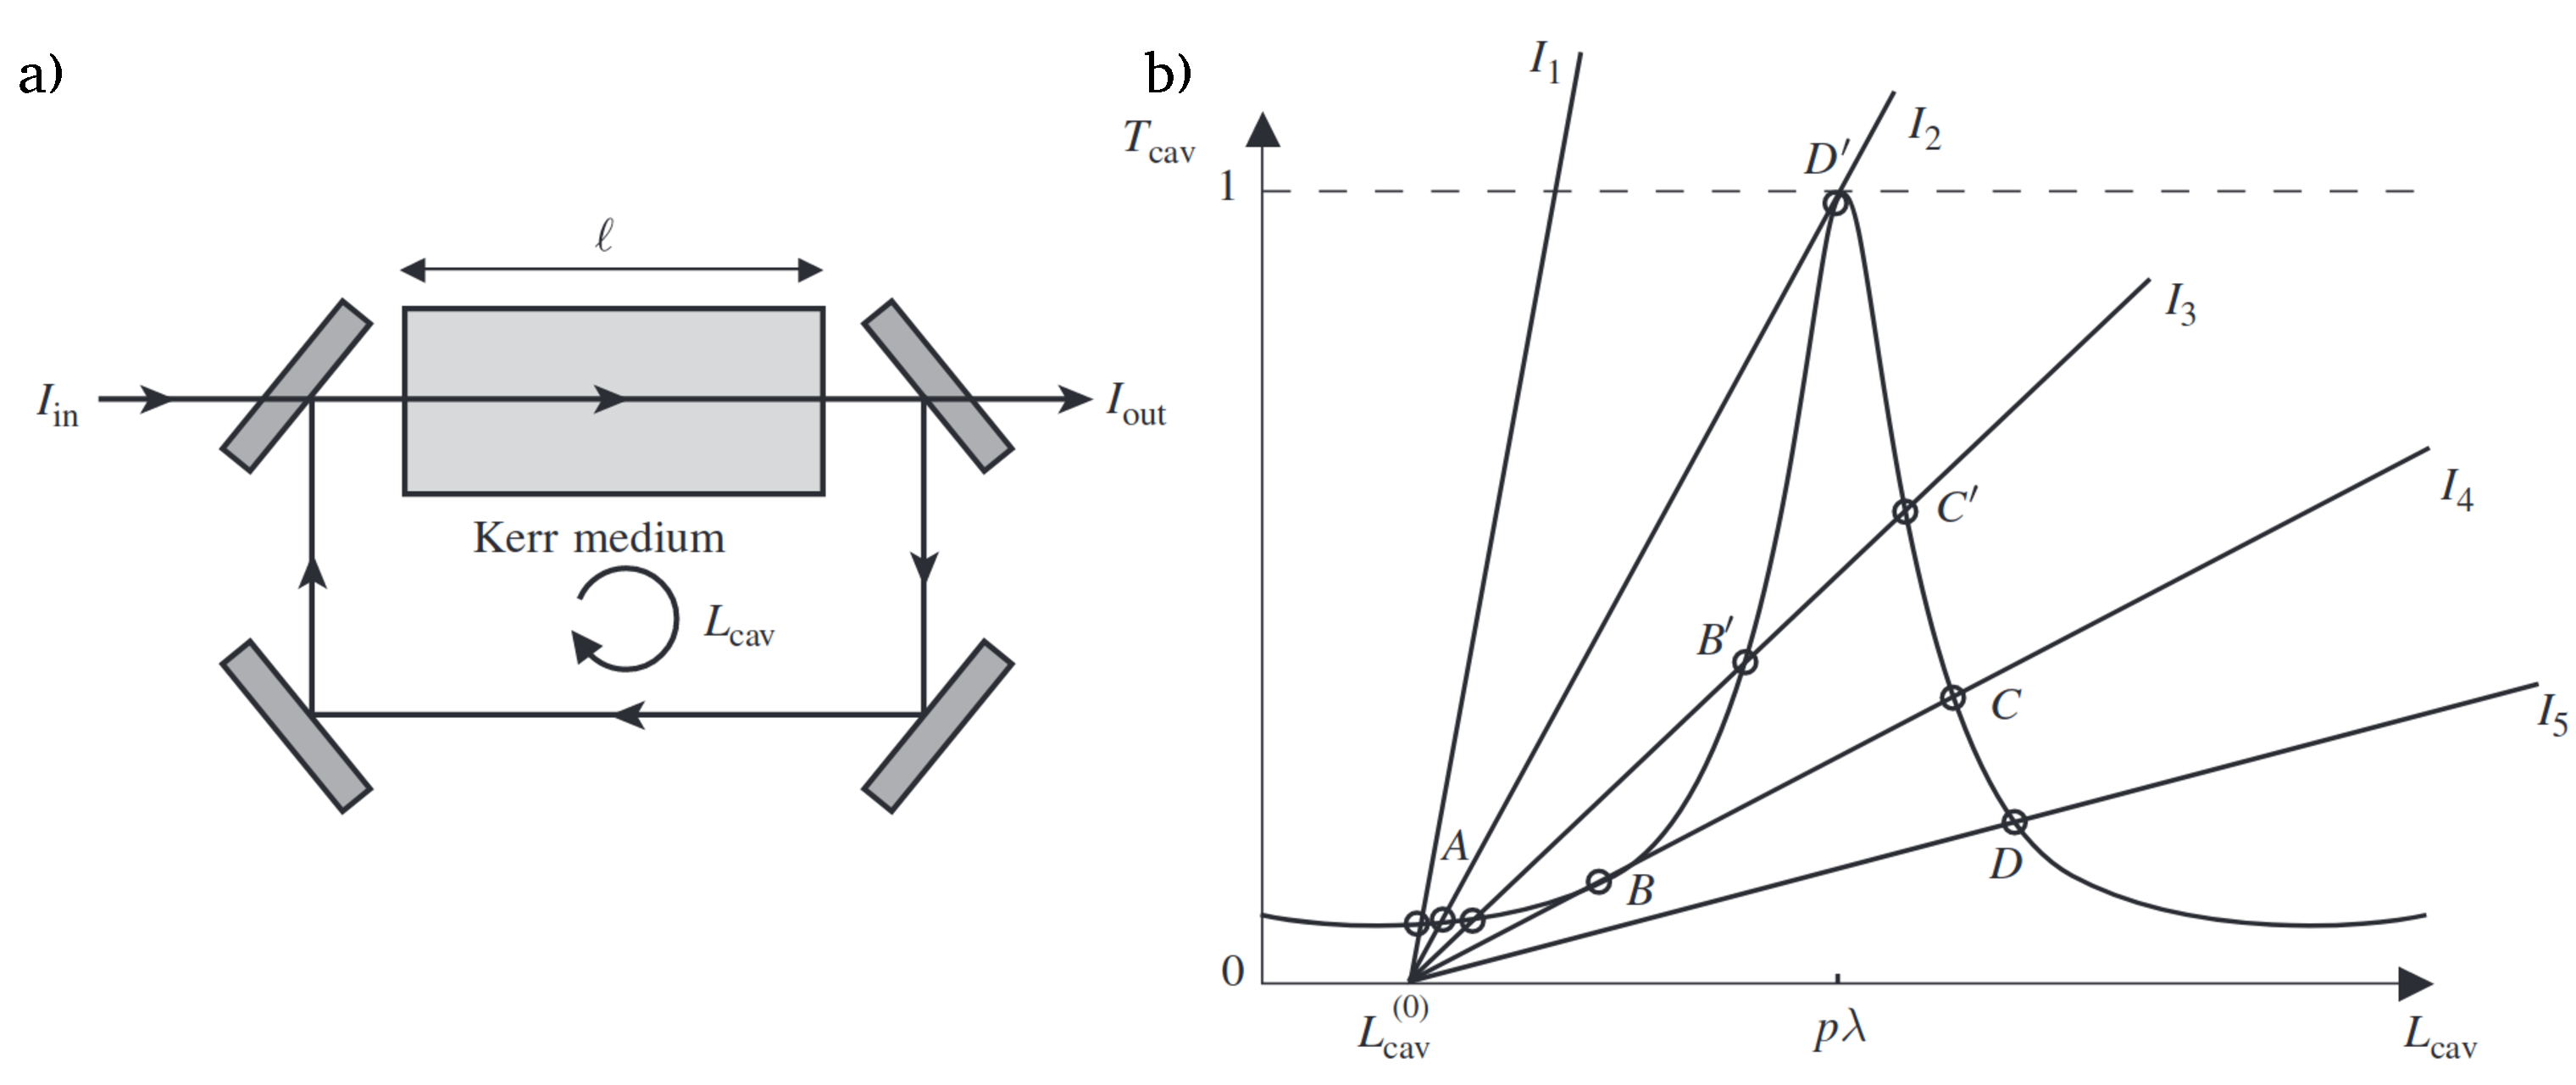
\includegraphics[width=1\linewidth]{chap_theory/fig/bistability_grynberg.pdf}
    \caption{\textbf{Optical bistability.} \textbf{a)} Schematic of a ring cavity filled with a Kerr medium. The cavity has a length $L_{cav}^{(0)}$ and the Kerr medium a length $l$. \textbf{b)} Transmission of the cavity as a function of the optical length of the cavity $L_{cav}$. The straight line represent the values $T_{cav}$ as a function of $L_{cav}$ for different values of
    $I_{in}$. The operating points lie at the intersections of the cavity resonance curve and the straigth lines. Depending on $I_{in}$ one or three operating point can be found. Adapted from \cite{grynberg_aspect_fabre}.}
    \label{fig:optical_bistability}
\end{figure}

To avoid first complications due to cross Kerr effect we consider a ring cavity of geometrical length $L$ filled with Kerr medium of lenght $l$ as shown in \autoref{fig:optical_bistability} a). The optical length of
such a cavity is :

\begin{equation}
    L_{cav}= L+(n_0-1)l+n_2I_{cav}l,
    \label{eq:optical_length}
\end{equation}
where $n_0$ is the refractive index of the medium, $n_2$ the non linear refractive index and $I_{cav}$ the intracavity intensity.
As explained for a planar cavity in \autoref{sec:photon}, the cavity has transmission peaks whenever the optical path of a round trip in the cavity (a photon going back and forth) is an integer multiple of the laser wavelength $\lambda$.
In the case of a ring cavity this condition reads as :

\begin{equation}
    T_{cav} = \dfrac{1}{1+\dfrac{4F^2}{\pi^2}\mathrm{sin}^2\left(\dfrac{kL_{cav}}{2}\right)},
    \label{eq:ring_cavity_transmission}
\end{equation}
where $F$ is the cavity finesse and $k=2\pi/\lambda$ the wavevector of the laser. The transmission of the cavity as a function of $L_{cav}$ is plotted in \autoref{fig:optical_bistability} b). 
On the other hand the transmission of the cavity is defined as :
\begin{equation}
    T_{cav} = \dfrac{I_{out}}{I_{in}}= T\dfrac{I_{cav}}{I_{in}}= \dfrac{T}{n_2l}\dfrac{L_{cav}-L^{(0)}_{cav}}{I_{in}},
    \label{eq:linear_transmission}
\end{equation}
where $T$ is the transmission of the outpout mirror and $L_{cav}^{(0)}$ the optical length of the cavity at low intensity $I_{cav}\approx 0$. An operating point is then defined as the intersection of the transmission curve \autoref{eq:ring_cavity_transmission} and the straight line of \autoref{eq:linear_transmission}. Graphically the slope 
of the linear relation between $T_{cav}$ and $L_{cav}$ depend on the value of $I_{in}$.
As a consequence several regime are possible depending on the value of the input intensity as shown in \autoref{fig:optical_bistability} b). For low intensity as $I_1$, the operating point is unique and the system is in a stable regime but yields a low transmission. For higher input intensity like $I_3$, the system exhibits three operating points. However, it can be shown that the intersection points with a negative derivative between B and D are unstable. At even higher 
intensity the system has again a single operating point and a poor transmission. When the input intensity lies between $I_2$ and $I_4$ the system is said to be in a bistable regime. 

\bigskip 

In the case of microcavity-polariton the same behavior can be observed as the exciton-exciton non-linear interactions are of the same nature as the Kerr effect.
Analytically, polariton bistability can be found by looking at the steady state of the driven-dissipative Gross-Pitaevskii equation in the presence of a driving pump term nearly resonant with the LP branch. In first approximation, it can be written as a plane wave $F_p(\rvec,t)=F_p e^{i\kvec_p.\rvec-i\omega_p t}$.
As it is usually done for equations including a resonant forcing term, we look for solution of the same form namely, plane wave with the same phase, $\psi(\rvec,t)= \sqrt{n_0}e^{i\kvec_p.\rvec-i\omega_p t}$.
Inserting this ansatz into \autoref{eq:generalized_GPE} in the absence of external potential $V_{LP}=0$ one obtain the steady state equation :

\begin{equation}
    \left[\omp -\omlp - \dfrac{\hbar \kp^2}{2 \mlp} - g n_0 - g_rn_r + i \dfrac{\gamlp}{2} \right] \sqrt{n_0}= \eta_{LP} F_p^0,
    \label{eq:steady_state}
\end{equation}
while the reservoir rate equation gives :
\begin{equation}
    n_r = \dfrac{\gamma_{in}}{\gamma_r}n_0.
\end{equation}
To eliminate the reservoir density we follow the procedure done in \cite{stepanov_dispersion_2019} and introduce an effective interaction strenght $g_{e}=g+g_r\frac{\gamma_{in}}{\gamma_r}$ so that $g_rn_r+gn=g_{e}n$. 
We can then rewrite \autoref{eq:steady_state} as :
\begin{equation}
    \left[\omp -\omlp - \dfrac{\hbar \kp^2}{2 \mlp} - g_{e}n_0 + i \dfrac{\gamlp}{2} \right] \sqrt{n_0}= \eta_{LP} F_p^0.
    \label{eq:steady_state_2}
\end{equation}
It is the equivalent of the equation of state of a conservative system with the difference that, in this case, it results of a complex equilibrium between interactions, pumping and losses. Notice that 
the contribution of the dark reservoir just appear as a correction on the interaction strength and thus doesn't change much the phenomenology discussed earlier. Nonetheless, it 
 has quantitative consequences on the hysteresis cycle that can be used to probe polariton-dark excitons interactions with optical means, notably through two photon excitation to overcome spin forbidden transitions \cite{dark_exciton_pol_interactions}

\bigskip

To end up with an equation linking the pump intensity to the polariton density one can multiply this equation by its complex conjugate which gives :

\begin{equation}
    n \left[ \dfrac{\gamlp^2}{4} + \left(\delta(\kp) - g_{e} n \right)^2 \right] =  \eta_{LP}^2 I,
\label{eq:eq_of_state}
\end{equation}

where $\delta(\kp)$ is the effective detuning between the pump laser and the LP branch at the pump wavevector in a parabolic approximation, $\delta(\kp) = \omp - \omlp-{\hbar\kp^2}/2\mlp$ and $I$ the pump intensity. Being a polynomial of degree 3 in the polariton density, this equation have up to three solutions.
Three distinct real solutions can be found only if $\delta>\sqrt{3/2}\gamlp$, as explained in the previous paragraph, one of this solution is known to be unstable. However, in some peculiar cases, namely when the fluid dimension is ramped down from 2D to 1D this solution can be explored and is responsible for the emergence of first order phase transition as investigated in \cite{li_dissipative_2022}.
This being said, we don't take into account this solution in the present work since the dimension of the fluid will always be 2D.
The evolution of $n$ as a function of $I$ in this regime is plotted in \autoref{fig:bistability}. The system is in a bistable regime when the curve exhibits two stable solutions for a given intensity : one at low density and one at high density.
It's worth noticing that the actual state in which the system is depend on its past history. More precisely, if the incident intensity is initially low, since the laser is blue detuned with the polariton energy, the photon injection whithin the sample is poor and a few polariton are created. However, their presence in the cavity tends to blueshift their own resonance energy as explained in \autoref{sub:polariton_interactions}. As the intensity is ramped up, the system will follow the low density branch until the energy renormalisation is sufficient to reach the point B. At this point the system is compelled to jump to the high density branch and will suddenly move from point B to point C.
If the pump intensity is then decreased, the situation is rather different since many polaritons are already present in the sample and support the laser injection and thus polariton creation. The system will follow the high density branch untill it reaches the point D' where interactions can no longer compensate for the losses making it fall again on the low density branch. A particular attention must be given to this so called turning point D'. Indeed, as it can be seen on \autoref{fig:optical_bistability} it's the only point at which the laser is exactly resonant with the cavity filled with non linearities.
This point can only be reached by travelling on the whole hysteresis loop. The corresponding density can determined by solving $\frac{dI}{dn}=0$ which gives the discriminants :

\begin{equation}
    \Delta = g_{e}^2 \left( \delta^2 - \dfrac{3\gamlp^2}{2}\right).
\end{equation}

The bistable regime require two distinct solution for $\frac{dI}{dn}=0$ which require $\Delta>0$ and provide the afromentionned condition $\delta>\sqrt{3/2}\gamlp$.
From this one can find that the density corresponding to the turning point fulfill $\delta(\kp)=g_{eff}n = gn_0+g_rn_r$. 

\begin{figure}
    \centering
    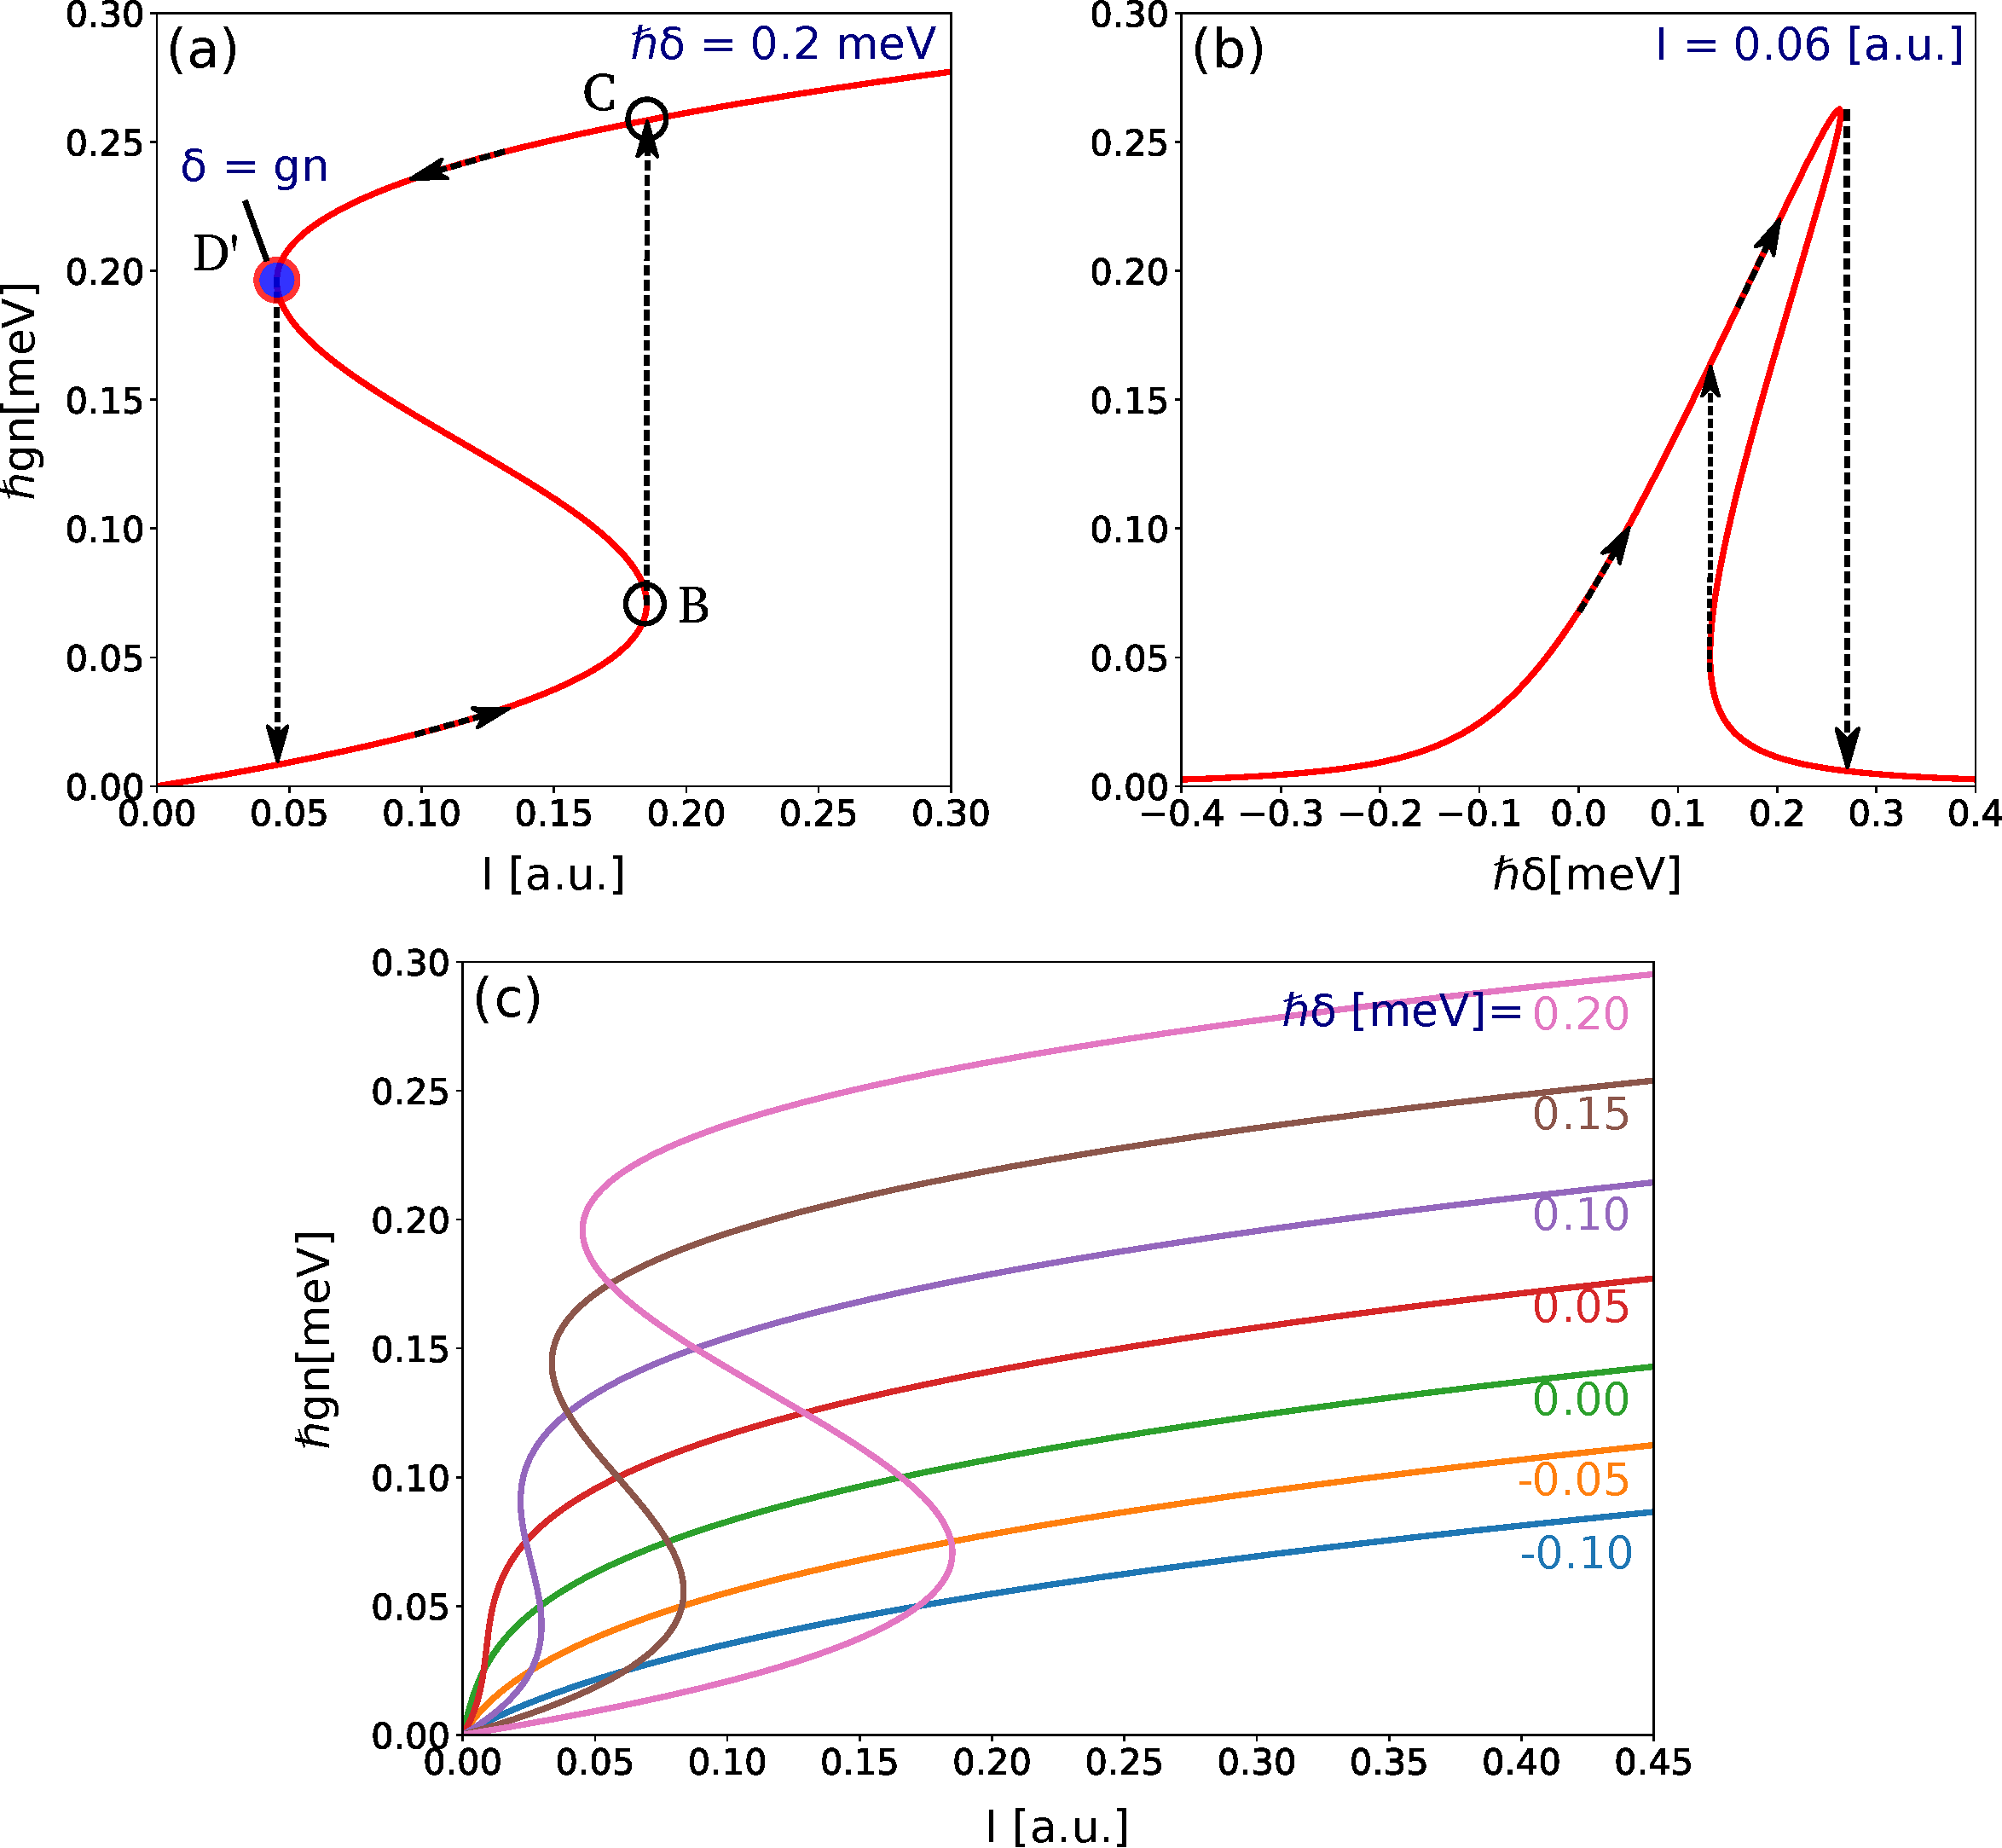
\includegraphics[width=0.8\linewidth]{chap_theory/fig/bistability.pdf}
    \caption{\textbf{Optical bistability in a polariton fluid.} \textbf{a)} The polariton density as a function of the pump intensity when $\delta>\frac{\sqrt{3}\gamlp}{2}$. The blue point represent the so called turning point at which the detuning is exactly equal to the interaction energy.
    \textbf{b)} Polariton density as a function of $\delta$ for a fixed pump intensity. c) Polariton density as a function of the pump intensity for different values of $\delta$, bistability is observed when $\delta>\frac{\sqrt{3}\gamlp}{2}$.}
    \label{fig:bistability}
\end{figure}

Conversely, when the detunig is two small with respect to the system losses the system is monostable and said to be in the optical limiter regime.
In the bistable regime, the system exhibits 


\textbf{All optical control.} In the context of analog gravity, the ability to easily control and monitor the fluid of light is a great asset. Indeed, the study of 
Hawking radiation in a quantum fluid require the creation of an acoustic horizon as well as the possibility to measure what is emitted by the latter. In particular,
it is crucial to achieve two goals. 

\begin{itemize}
    \item 1. Create and monitor a stable fluid with an arbitray flow profile and density since the mean field and especially its velocity profile are the analog of the curved spacetime we want to study.
    \item 2. Probe the fluid collective excitations. These small perturbations on top of the mean field are the fluid counterpart of the quantum fields fluctuations considered in the Hawking radiation theory.
\end{itemize}

With planar microcavity polaritons this is done fully optically since the fluid is created by the pump laser and is monitored by collecting the photons leaving the sample. 
The first point is allowed by the resonant excitation scheme. The velocity of a polariton being $\mathbf{v_{LP}}=\frac{\hbar \kvec_{LP}}{\mlp}$ momentum conservation enable to create a fluid with a given velocity by just changing the pump incidence angle (see \autoref{sec:photon}).
This correspondance also holds for the light outgoing the sample : the recombination of a polariton with wavevector $\kvec$ produce a photon with the same wavevector. 
Although the relation between the pump intensity and the polariton density is not trivial as we shall see in the next section, it is also a practical control knob that can be used to tune the fluid speed of sound.
The second point can again be tackled with optics means since the struture of collective excitations is ultimately hidden in the fluctuations of the photonic field outgoing the sample. As a consequence, the large
variety of tools and methods developped in the field of optics can be used to probe the fluid. Microcavity polaritons, are liying at the crossroad of optics and quantum fluids, definitely justifying the designation "quantum fluid of light".
